
%\documentclass[sigconf,review, anonymous]{acmart}
\documentclass[10pt,conference]{IEEEtran}
\usepackage{dblfloatfix}
\usepackage{graphicx}
\usepackage[colorinlistoftodos]{todonotes}
\usepackage{blindtext, graphicx}
\usepackage{hyperref}
\usepackage{caption}
\usepackage{cite}
\usepackage{float}
\usepackage{balance}
\usepackage{listings}
\renewcommand\thesection{\arabic{section}}
%\renewcommand\thesubsection{\thesection\arabic{subsection}}
\usepackage{amsmath}
\usepackage{tikz}
\usepackage{comment}
\usepackage{framed}
\usepackage{multirow}
\usepackage{rotating}
\usepackage{bigstrut}
\usepackage{color}
\usepackage{eqparbox}
\usepackage{graphics}
\usepackage{colortbl}
\usepackage{paralist}
\usepackage{algorithm}
\usepackage{algorithmicx}
\usepackage{algpseudocode}
\usepackage{mathptmx} 
\usepackage{picture}
\usepackage[shortlabels]{enumitem}
\usepackage{url}
\usepackage{pifont}% http://ctan.org/pkg/pifont

\newcommand{\cmark}{\ding{51}}%
\newcommand{\xmark}{\ding{55}}%

\newcommand{\bi}{\begin{itemize}[leftmargin=0.4cm]}
	\newcommand{\ei}{\end{itemize}}
\newcommand{\be}{\begin{enumerate}}
	\newcommand{\ee}{\end{enumerate}}

\usepackage{tabularx}
\usepackage{colortbl}
\usepackage{hhline}
\usepackage[export]{adjustbox}
\definecolor{lightgray}{gray}{0.8}
\definecolor{darkgray}{gray}{0.6}
\definecolor{lavenderpink}{rgb}{0.98, 0.68, 0.82}
\definecolor{celadon}{rgb}{0.67, 0.88, 0.69}
\renewcommand{\algorithmicrequire}{\textbf{Input:}}
\renewcommand{\algorithmicensure}{\textbf{Output:}}
%%% graph
\newcommand{\crule}[3][darkgray]{\textcolor{#1}{\rule{#2}{#3}}}

\newcommand{\quart}[4]{\begin{picture}(80,4)%1
	{\color{black}\put(#3,2){\circle*{4}}\put(#1,2){\line(1,0){#2}}}\end{picture}}

\definecolor{Gray}{gray}{0.95}
\definecolor{LightGray}{gray}{0.975}

\definecolor{steel}{rgb}{.11, .11, .7}
\definecolor{Gray}{rgb}{0.88,1,1}
\definecolor{Gray}{gray}{0.85}
\usepackage[framed]{ntheorem}
\usetikzlibrary{shadows}
\theoremclass{Lesson}
\theoremstyle{break}

% inner sep=10pt,
\tikzstyle{thmbox} = [rectangle, rounded corners, draw=black,
fill=Gray!40,  drop shadow={fill=black, opacity=1}]
\newcommand\thmbox[1]{%
	\noindent\begin{tikzpicture}%
	\node [thmbox] (box){%
		\begin{minipage}{.94\textwidth}%
		\vspace{-2mm}#1\vspace{-1mm}%
		\end{minipage}%
	};%
	\end{tikzpicture}}

\let\theoremframecommand\thmbox
\newshadedtheorem{lesson}{Result}

\theoremclass{Lesson1}
\theoremstyle{break}

\let\theoremframecommand\thmbox
\newshadedtheorem{lesson1}{Result}
\newcommand{\tion}[1]{{\S}\ref{sect:#1}}

\usepackage{listings}
\definecolor{MyDarkBlue}{rgb}{0,0.08,0.45} 
\lstset{
    language=Python,
    basicstyle=\sffamily\fontsize{3mm}{0.8em}\selectfont,
    breaklines=true,
    prebreak=\raisebox{0ex}[0ex][0ex]{\ensuremath{\hookleftarrow}},
    frame=l,
    keepspaces=false,
    showtabs=false,
    columns=fullflexible,
    showspaces=false,
    showstringspaces=false,
    keywordstyle=\bfseries\sffamily,
    emph={ m, r, k, frontier, cf, f, g, n}, emphstyle=\bfseries\color{blue!50!black},
    stringstyle=\color{green!50!black},
    commentstyle=\color{red!50!black}\it,
    numbers=left,
    captionpos=t,
    escapeinside={\%*}{*)}
}

\DeclareMathOperator\caret{\raisebox{0.4ex}{$\scriptstyle\wedge$}}


\newcommand{\sma}{{\sc SMOTE}}
\newcommand{\smb}{{\sc SMOTUNED}}

\begin{document}

\pagestyle{plain}

\title{``Better Data'' is Better than ``Better Data Miners''\\ (Benefits of Tuning SMOTE for Defect Prediction) }

% \author{Amritanshu Agrawal, Tim Menzies\\
% Computer Science, NC State, USA\\
% aagrawa8@ncsu.edu, tim@menzies.us
% }


%\author{Author name(s) blinded for review.}
\author{\IEEEauthorblockN{Amritanshu Agrawal}
\IEEEauthorblockA{Department of Computer Science\\
North Carolina State University\\
Raleigh, NC, USA\\
Email: aagrawa8@ncsu.edu}
\and
\IEEEauthorblockN{Tim Menzies}
\IEEEauthorblockA{Department of Computer Science\\
North Carolina State University\\
Raleigh, NC, USA\\
Email: tim@menzies.us}}

\maketitle

\begin{abstract}
We report and fix an important systematic error in prior
studies that ranked classifiers for software analytics.
Those studies  did  not (a)~assess classifiers on multiple   criteria
and they did not 
(b)~study  how variations in the  data affect the results. 
Hence, 
this paper applies (a)  multi-criteria tests while (b)~fixing the weaker regions of the training
 data (using {\smb}, which is a self-tuning version of {\sma}).
This approach
leads to dramatically large increases in software defect predictions.
When applied in a 5*5 cross-validation study for  3,681	JAVA classes (containing over a million lines of code) from open source  systems,
{\smb} increased
AUC and recall by 60\% and 20\% respectively. 
These improvements were independent of the classifier used to
predict for quality.

We hence conclude that, for  software analytics, (1)~data
pre-processing can be more important than  classifier
choice,
(2)~ranking studies  are  incomplete  without
 pre-processing and
(3)~{\smb} is a   promising candidate for  pre-processing.

\end{abstract}


%\keywords{
%Performance Prediction, SBSE, Sampling, Rank-based method}
\begin{IEEEkeywords}
Search based software engineering,
defect prediction, classification, 
data analytics for software engineering, SMOTE,  imbalanced data, preprocessing
\end{IEEEkeywords}

\IEEEpeerreviewmaketitle


\section{Introduction}
\label{sect:intro}
Software quality methods cost money and better quality costs exponentially more money~\cite{voas95,fu2016tuning}.  
Given finite budgets, quality assurance resources are usually 
skewed towards areas known to be most safety critical or mission critical~\cite{lowryBK98}. This leaves ``blind spots'': regions of the system that may contain defects which may be missed. Therefore, in addition to rigorously assessing  critical areas, a parallel activity should be to {\em sample the blind spots}~\cite{Menzies04}. 

For sampling those blind spots, many researchers  use  {\em static code defect predictors}.
%~\cite{lessmann2008benchmarking, hall2012systematic, elish2008predicting, pears2014synthetic, pelayo2012evaluating, tan2015online, kamei2007effects, pelayo2007applying, menzies2010defect, gondra2008applying, radjenovic2013software, jiang2008techniques, wang2013using, mende2009revisiting, li2012sample, khoshgoftaar2010attribute, jiang2009variance, ghotra2015revisiting, tantithamthavorn2016automated, fu2016tuning, jiang2008can,d2010extensive,menzies2007data, nagappan2006mining,shepperd2014researcher,Menzies2010,hassan2009predicting, kim2007predicting,song2011general, song2006software}.
Starting with source code divided into sections, researchers annotate the code with the number of issues known for each section.
Classification algorithms are then applied to learn what static code attributes
distinguish 
between sections with few/many issues.
Such static code measures can be automatically extracted from
the code base, with very little effort even for very large software
systems~\cite{Nagappan:2005}.  


One perennial problem   is what classifier should be applied to build the defect predictors?
To address this problem, numerous papers report {\em ranking studies} where
some quality measure  is collected from  several  classifiers when they are 
 applied to data sets.
For examples of such studies,
see~\cite{lessmann2008benchmarking,hall2012systematic,elish2008predicting,menzies2010defect,gondra2008applying,radjenovic2013software,jiang2008techniques,wang2013using,mende2009revisiting,li2012sample,khoshgoftaar2010attribute,jiang2009variance,ghotra2015revisiting,jiang2008can,tantithamthavorn2016automated,fu2016tuning}.
Such ranking studies conclude that some subset of the classifiers
are  ``best'' if they generate  better quality scores.
Our claim is that such conclusions are incomplete when
they ignore the impact of  
data pre-processing. As shown below,
a new data pre-processing method called {\smb}
 consistently generates better 
defect predictors,
{\em regardless of the classifier used
to make the predictions}.  


 \begin{figure*}[!t]
\renewcommand{\baselinestretch}{0.8}\begin{center}
{\scriptsize
\begin{tabular}{c|l|p{4.0in}}
amc & average method complexity & e.g. number of JAVA byte codes\\
\hline
avg, cc & average McCabe & average McCabe's cyclomatic complexity seen
in class\\
\hline
ca & afferent couplings & how many other classes use the specific
class. \\
\hline
cam & cohesion amongst classes & summation of number of different
types of method parameters in every method divided by a multiplication
of number of different method parameter types in whole class and
number of methods. \\
\hline
cbm &coupling between methods & total number of new/redefined methods
to which all the inherited methods are coupled\\
\hline
cbo & coupling between objects & increased when the methods of one
class access services of another.\\
\hline
ce & efferent couplings & how many other classes is used by the
specific class. \\
\hline
dam & data access & ratio of the number of private (protected)
attributes to the total number of attributes\\
\hline
dit & depth of inheritance tree &\\
\hline
ic & inheritance coupling & number of parent classes to which a given
class is coupled (includes counts of methods and variables inherited)
\\
\hline
lcom & lack of cohesion in methods &number of pairs of methods that do
not share a reference to an case variable.\\
\hline
locm3 & another lack of cohesion measure & if $m,a$ are the number of
$methods,attributes$
in a class number and $\mu(a)$ is the number of methods accessing an
attribute,
then
$lcom3=((\frac{1}{a} \sum, j^a \mu(a, j)) - m)/ (1-m)$.
\\
\hline
loc & lines of code &\\
\hline
max, cc & maximum McCabe & maximum McCabe's cyclomatic complexity seen
in class\\
\hline
mfa & functional abstraction & number of methods inherited by a class
plus number of methods accessible by member methods of the
class\\
\hline
moa & aggregation & count of the number of data declarations (class
fields) whose types are user defined classes\\
\hline
noc & number of children &\\
\hline
npm & number of public methods & \\
\hline
rfc & response for a class &number of methods invoked in response to
a message to the object.\\
\hline
wmc & weighted methods per class &\\
\hline
 
nDefects & raw defect counts & Numeric: number of defects found in post-release bug-tracking systems.\\
\rowcolor{lightgray}
defects present? & Boolean& if {\em nDefects} $>0$ then {\em true} else {\em false}
\end{tabular}
}
\end{center}
\caption{OO CK code metrics used for all studies in this paper.
The last line, shown in denotes the dependent variable.}
\label{fig:ck}
\vspace{-0.7cm}
\end{figure*}


{\smb} is an auto-tuning version of  {\sma}~\cite{chawla2002smote}, which is
a method for addressing the class imbalance problem. SE data
sets are often imbalanced; i.e. the data in the target class is overwhelmed by an over-abundance of information about everything else except the target~\cite{menzies2007problems}. To
address this problem, {\sma} under-samples
the majority class while intelligently super-sampling  the minority class. Standard
{\sma} is controlled by a default
set of parameters which {\smb} tunes 
for each new data set. 

To assess {\smb}, this paper explores defects from  3,681	 classes (containing over a million lines of code) from open source JAVA systems. We ask three research questions: 
 \bi\item
  \textbf{RQ1}:  {\em Are the default ``off-the-shelf'' parameters for {\sma} appropriate for
  all data sets?} 
  \ei
 \begin{lesson}{\smb} learned different parameters for each data set, all of which  were very different to default {\sma}.
 \end{lesson}
  \bi
  \item
  \textbf{RQ2}: {\em   Is  there any benefit in tuning the default parameters of {\sma} for
  each new data set?} 
  \ei
   \begin{lesson}After using {\smb}, the observed performance improvements are dramatically large; e.g. improvements in recall  up to 60\% against {\sma}.
 \end{lesson}
Some of these improvements are so very large that they overturn established wisdom in this find.
For example,  Ghotra et al.~\cite{ghotra2015revisiting} and Lessmann et al.~\cite{lessmann2008benchmarking}
 report that   random forest is a  good default choice for  defect predictors.
But with  {\smb}, random forest is usually
beaten by other classifiers. 

More generally, no learner was consistently ``best'' across all data sets and all performance criteria; yet {\smb} was consistently  used by  whatever  learner was found to be ``best''.  
That is,  creating better training data is more important
than the subsequent choice of a classifier.  To say that another way: ``better data'' is better than ``better data miners''.
 
% That is,  the improvements gained by
% {\smb} were  {\em  independent of the  classifier used to
% predict for defects}.
% This  result calls into question any prior ranking studies that  only considered the classifier {\em but not the data pre-processing applied before learning}.   
  
   \bi
  \item
  \textbf{RQ3}: {\em  In terms of runtimes, is the cost of running {\smb} worth the performance improvement?}
  \ei
  
   \begin{lesson}In the data studied here,
   {\smb} usually terminates in under two minutes; i.e.  fast enough
   to recommend its widespread use.
 \end{lesson}


\noindent
In summary, the  contributions of this paper are:
\bi
\item The discovery of an important systematic error in  many prior ranking studies; i.e., all of
~\cite{lessmann2008benchmarking,hall2012systematic,elish2008predicting,menzies2010defect,gondra2008applying,radjenovic2013software,jiang2008techniques,wang2013using,mende2009revisiting,li2012sample,khoshgoftaar2010attribute,jiang2009variance,ghotra2015revisiting,jiang2008can,tantithamthavorn2016automated,fu2016tuning}.
\item A novel application of search-based SE ({\smb});
\item Dramatically large improvements in  defect predictors;
\item Potentially, for any other software analytics task that uses classifiers, a way to improve those learners as well;
\item A methodology for assessing the value of pre-processing data sets in software analytics;
\item A reproduction package to reproduce our results then (perhaps) to improve or refute  our results\footnote{Available to download from https://github.com/ai-se/Smote\_tune},
\ei
The rest of this paper is structured as follows:
\tion{review} gives an overview on software defect prediction.
\tion{performance} talks about all the performance criteria used in this paper.
\tion{imbalance} explains the problem of class imbalance in defect prediction. Assessment of the previous ranking studies is done in \tion{rank}.
\tion{smote} introduces {\sma} and discusses how {\sma} has been used in literature. \tion{smotuned} provides the definition of {\smb}. The experimental setup of this paper is discussed in \tion{experiment}.
We have answered above research questions in
\tion{results}. This is followed by a discussion on the validity of our results 
and a section describing our conclusions.
 

% \item \textbf{RQ3}: \textbf{Should SMOTE be used ``off-the-shelf'' with their default tunings?}

 

%We created a python package generalised to run any CK metrics based dataset and compare results against 6 learners. Since the classes are imbalanced we used SMOTE~\cite{chawla2002smote} (only on Training Data) which is a synthetic minority over-sampling technique.

%The remainder of the paper is organized as follows. Section \ref{review} gives a brief related work on defect prediction. Section \ref{motivation} talks about why there is a need to balance the data. Since we found astonishing results with smote, section \ref{smote} talks about SMOTE in defect prediction. Experimental setup is provided in section \ref{experiment}. Results are discussed in Section \ref{results}. Threats to validity section is discussed in section \ref{validity}. Final conclusion is being discussed in section \ref{conclusion}. And section \ref{future} talks about our future work.

 


\section{Background and Motivation}

\subsection{Defect Prediction}
\label{sect:review}

There is a long tradition in software engineering of trying to find undiscovered defects in software. 
Hall et al.~\cite{hall2012systematic} surveyed some of the methods
applied to this task: statistical approaches, capture-recapture 
(CR) models, detection profile methods (DPM)~\cite{song2011general} or
association rule mining~\cite{song2006software}. 

A variety of approaches have been proposed to recognize
 defect-prone  software components using code metrics (lines of code, complexity)~\cite{d2010extensive,menzies2007data, nagappan2006mining,shepperd2014researcher,Menzies2010}, process metrics (number of changes, recent activity)~\cite{hassan2009predicting} or previous defects~\cite{kim2007predicting}.
Other work, such as that of 
Bird et al.~\cite{bird2009putting}, indicated that it is possible to predict which components (for example modules) are likely locations of
defect occurrence using a component's development history,
and dependency structure. 
% Two key properties of software components
% in large systems are dependency relationships (which components
% depend on or are dependent on by others), and development
% history (who made changes to the components and
% how many times). Thus, we can link software components
% to other components i) in terms of their dependencies, and
% also ii) in terms of the developers that they have in common.
Prediction models based on the topological properties
of components within them have also  proven to be  
accurate~\cite{zimmermann2008predicting}.

The lesson of all the above  is that the probable location
of future defects can be guessed using   logs of past defects~\cite{hall2012systematic, catal2009systematic}. These logs might
summarize software components using
static code metrics such as 
McCabes  cyclomatic  complexity, Briands coupling metrics, code metrics,  
dependencies between  binaries, or
the  CK  metrics  suite~\cite{chidamber1994metrics} described in  Figure~\ref{fig:ck}. 
One advantage with CK metrics is that they are  simple  to  compute and hence,
they are widely used. Radjenovi{\'c} et al.~\cite{radjenovic2013software} report that in
the static code defect prediction, the CK metrics are
used  twice as much (49\%) 
as more traditional source code metrics such as McCabes (27\%) or process metrics (24\%).

Using these CK metrics, building such static code defect predictors is remarkably fast and rapid process.
Given the current generation of data mining toolkits, it can be a matter
of just a few seconds to learn a defect predictor (see the runtimes in Table~9 of reference~\cite{fu2016tuning}). Further, in a recent study at ICSE'14, Rahman et
al.~\cite{Rahman14} found no significant differences in the cost-effectiveness
of
(a) static code analysis tools FindBugs, and Jlint and (b) static code defect predictors.
This is an interesting result since it is  much slower to adapt static code
analyzers to new  languages than defect predictors (since the latter just requires hacking together some new
static code metrics extractors).

\subsection{Performance Criteria}
\label{sect:performance}

%\begin{figure}[!htpb]
%    \centering
%    \includegraphics[scale=0.35]{cmatrix.png}
%    \caption{Confusion Matrix}%

%    \label{fig:cmatrix}
%\end{figure}

Formally, defect prediction is a binary classification problem.
The performance of a defect predictor can be assessed via a  confusion matrix like Table~\ref{fig:cmatrix}
where a ``positive'' output is the defective class under study and a ``negative'' output is the non-defective one.
Further, ``false'' means the learner got it wrong and ``true'' means the learner correctly identified
a fault or non-fault module. Hence, Table~\ref{fig:cmatrix} has four quadrants containing, e.g $\mathit{FP}$ which denotes ``false positive''.


\begin{table}[!h]
\scriptsize
\begin{center}
\begin{tabular} {@{}cc|c|c|l@{}}
\cline{3-4}
& & \multicolumn{2}{ c| }{Actual} \\ \cline{3-4}
& & defect-free & defective  \\ \cline{1-4}
\multicolumn{1}{ |c  }{\multirow{2}{*}{Prediction} } &
\multicolumn{1}{ |c| }{defect-free} & $\mathit{TN}$ & $\mathit{FN}$ & \\ \cline{2-4}
\multicolumn{1}{ |c  }{}                        &
\multicolumn{1}{ |c| }{defective} & $\mathit{FP}$& $\mathit{TP}$  &  \\ \cline{2-4}
\cline{1-4}
\end{tabular}
\caption{Confusion Matrix}
\label{fig:cmatrix}
\end{center} 
\vspace{-0.6cm}
\end{table}


From this matrix, we can define performance measures like   \textbf{Area Under Curve (AUC)}, which 
is the area covered by an ROC curve~\cite{swets1988measuring, duda2012pattern} in which the X-axis represents
\[\mathit{FPR} = \mathit{FP}/(\mathit{FP} + \mathit{TN})\]
and the Y-axis represents:
\[\mathit{TPR} = \mathit{TP}/(\mathit{TP} + \mathit{FN})\]
\textbf{Recall}  is the fraction of  relevant instances that are retrieved:
\[Recall= pd  = \mathit{TP}/(\mathit{TP} + \mathit{FN})\]
 \textbf{Precision} is the fraction of retrieved instances that are relevant:
\[Precision  = prec = \mathit{TP}/(\mathit{TP} + \mathit{FP})\]
\textbf{False Alarm} is the ratio of false positive to total predicted negative:
\[False\ alarm = pf  = \mathit{FP}/(\mathit{FP} + \mathit{TN})\]
As shown in Figure~\ref{fig:trade},
a typical predictor must ``trade-off''
between false alarm and recall.
This is because the  more sensitive the detector, the more often it triggers and the higher its recall. On the other hand,  if a detector triggers more often, it can also raise more false alarms.
Hence, when increasing recall, we  should  expect
the false alarm rate to  increase
(ideally, not by very much).


\begin{figure}[!b]
\begin{center}
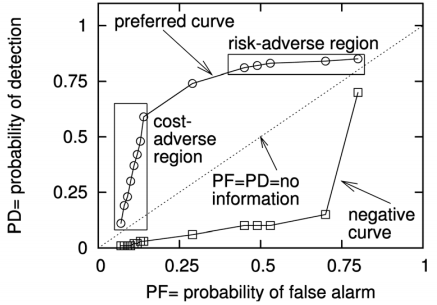
\includegraphics[width=2.5in]{roc.png}
\end{center}
\caption{Trade-offs false alarm vs
recall (probability of detection). Dotted line shows where false alarm is as common as detecting the signal.
The {\em negative curve} is for models where, if something is negated, performance flips  to the top-left region. }\label{fig:trade}
\end{figure}

There are many more ways to evaluate defect predictors besides the four listed above
(see Table 23.2 of~\cite{menzies2014sharing} for   eleven additional
criteria seen in the current software analytics literature).
No evaluation criteria is ``best'' since different  criteria are appropriate in different business contexts. For example, as shown
in 
Figure~\ref{fig:trade},
when dealing
with safety-critical applications, management may be
``risk adverse'' and hence many elect
 to {\em maximize recall}, regardless of the time wasted exploring  false alarm.
 Similarly, 
when rushing some non-safety critical application to market, management may be ``cost adverse''
and elect to {\em minimize false alarm} since this avoids distractions to the developers. 
 Accordingly, it is a good practice to evaluate defect predictors on more than a single performance criterion. For example, in this paper,
we use all the four   criteria listed above
(and we use four since they have
been used in recent papers  
at prominent SE conferences~\cite{ghotra2015revisiting} and SE journals~\cite{fu2016tuning}).
 

\subsection{Defect Prediction and Class Imbalance}
\label{sect:imbalance}

Class imbalance learning refers to learning from datasets that exhibit significant imbalance among or within classes. Class imbalance  is concerned with the situation in where some classes of data are
highly under-represented compared to other classes~\cite{he2009learning}.
By convention,
the under-represented class is called the {\em minority} class,
and correspondingly the class which is over-represented is called the
{\em majority} class. In this paper, we say that class imbalance is {\em worse}
when the ratio of minority class to majority {\em increases}, that is,
{\em class-imbalance of 5:95} is worse than {\em 20:80}. Menzies et al.~\cite{menzies2007problems} reported SE data sets often contain class imbalance. In their examples, they showed static code defect prediction data sets with
class imbalances of 1:7; 1:9; 1:10; 1:13; 1:16; 1:249.
They also show mathematically that  class imbalances  have a very large  negative effect on the performance of static code defect predictors.  

The problems of class imbalance are sometimes discussed in the software analytics community.
Hall et al.~\cite{hall2012systematic} found that models based on C4.5 under-perform if they have imbalanced data while Naive Bayes and Logistic regression perform relatively better. 
Their general recommendation is to not use
imbalanced data.  
Some researchers offer preliminary explorations into methods that might mitigate for class imbalance.
Wang et al.~\cite{wang2013using} and Yu et al.~\cite{yuperformance} validated the Hall et al. results and concluded that the
performance of C4.5 is unstable on imbalanced datasets while  Random Forest and Naive Bayes are 
more stable. 
Yan et al.~\cite{yan2010software} performed fuzzy logic and rules to overcome the imbalance problem, but they only
explored one kind of learner (Support Vector Machines).
Pelayo et al.~\cite{pelayo2007applying} studied the effects of the percentage of oversampling and undersampling done. They found out that different percentage of each helps improve the accuracies of decision tree learner for defect prediction using CK metrics. Menzies et al.~\cite{menzies2008implications} undersampled the non-defect class to balance training
data and reported how little information was required to learn a defect predictor. They found that throwing away data does not degrade the performance of Naive Bayes and C4.5 decision trees. Other papers show the usefulness of resampling based on different learners~\cite{pelayo2007applying, pelayo2012evaluating, riquelme2008finding}.

We note that  
many researchers in this area  (Wang, Yu et al, Gray et al.~\cite{gray2009using,yuperformance,wang2013using} refer to the {\sma} method explored in this paper,  but only in the context of future work. 
Also, 
in this sample, no researcher has  applied auto-tuning to learn best {\sma} control parameters. 
 

\subsection{Ranking Studies}
\label{sect:rank}

A constant problem in defect predictions is what  classifier should be applied to  build  the  defect  predictors?
To address this problem, many researchers run {\em ranking studies} where  performance scores 
are collected from  many classifiers  executed on  many software defect data sets~\cite{lessmann2008benchmarking,hall2012systematic,elish2008predicting,menzies2010defect,gondra2008applying,radjenovic2013software,jiang2008techniques,wang2013using,mende2009revisiting,li2012sample,khoshgoftaar2010attribute,jiang2009variance,ghotra2015revisiting,jiang2008can,tantithamthavorn2016automated,fu2016tuning}.
This section assesses those ranking studies. We will say a ranking study is ``good'' if it compares multiple learners using multiple data sets and multiple evaluation criteria
while at the same time doing something to address the data imbalance problem.

 In February  2017,  we searched
scholar.google.com for the conjunction of ``software'' and ``defect prediction'' and ``oo'' and ``ck'' published in the last decade. This returned 231 results.
From that list, we selected ``highly-cited'' papers, which we defined as having more than 10 citations per year.  This reduced our population of papers down to 107.
After reading the titles and abstracts of those papers, and skimming the contents of the potentially interesting papers, we found 22 papers of Table~\ref{tbl:survey2} that either performed ranking studies
(as defined above) or studied the effects of class imbalance on defect prediction. In the column ``evaluated using
multiple criteria'',
papers scored more than ``1'' if they used multiple performance scores  of the kind listed at the end of \tion{performance}. 

 \begin{table}[!htbp]
\scriptsize
\centering
    \begin{tabular}{c@{~}|c@{~}|c@{~}|c@{~}|c@{~}|c@{~}}
        \begin{tabular}[c]{@{}c@{}}\textbf{ref}\end{tabular} & \textbf{Year} & \textbf{Citations} & \begin{tabular}[c]{@{}c@{}}\textbf{Ranked} \\\textbf{Classifiers?} \end{tabular} &\begin{tabular}[c]{@{}c@{}} \textbf{Evaluated} \\\textbf{using} \\\textbf{multiple} \\\textbf{criteria?}\end{tabular}&\begin{tabular}[c]{@{}c@{}} \textbf{Considered}\\\textbf{Data Imbalance?} \end{tabular}\\ \hline
        \cite{lessmann2008benchmarking} & 2008 & 575 & \cmark & 1 & \xmark \\ 
        \cite{hall2012systematic} & 2012 & 359 & \cmark & 3 & \xmark \\
        \cite{elish2008predicting} & 2008 & 281 & \cmark & 4 & \xmark\\  
        \cite{menzies2010defect} & 2010 & 170 & \cmark & 1 & \xmark \\  
        \cite{gondra2008applying} & 2008 & 153 & \cmark & 1 & \xmark\\     
        \cite{Kim:2011} & 2011 & 141 &\xmark & 1 & \cmark \\ 
        \cite{radjenovic2013software} & 2013 & 133 & \cmark & 1 & \xmark \\   
        \cite{jiang2008techniques} & 2008 & 127 & \cmark & 5 & \xmark \\    
        \cite{menzies2007problems} & 2008 & 126 & \cmark & 1 & \cmark \\   
        \cite{wang2013using} & 2013 & 94 & \cmark & 1 & \cmark \\  
        \cite{mende2009revisiting} & 2009 & 90 & \cmark & 1 & \xmark \\          
        \cite{li2012sample} & 2012 & 72 & \cmark & 3 & \xmark  \\ 
        \cite{kamei2007effects} & 2007 & 69 & \xmark & 3 & \cmark\\  
        \cite{pelayo2007applying} & 2007 & 58 & \xmark & 1 & \cmark \\  
        \cite{khoshgoftaar2010attribute} & 2010 & 57 & \cmark & 1 & \cmark  \\  
        \cite{jiang2009variance} & 2009 & 57 & \cmark & 4 & \xmark  \\  
        \cite{ghotra2015revisiting} & 2015 & 43 & \cmark & 1 & \xmark  \\  
        \cite{jiang2008can} & 2008 & 39 & \cmark & 1 & \cmark  \\  
        \cite{tan2015online} & 2015 & 23 & \xmark & 3 & \cmark \\  
        \cite{pelayo2012evaluating} & 2012 & 23 & \xmark & 1 & \cmark \\  
        \cite{tantithamthavorn2016automated} & 2016 & 21 & \cmark & 1 & \xmark\\  
        \cite{fu2016tuning} & 2016 & 12 & \cmark & 2 & \xmark  \\    
\end{tabular}
\caption{22 highly cited ranking studies.}
\label{tbl:survey2}
\vspace{-0.5cm}
\end{table}

 \begin{table*}[!htbp]
 \begin{tabular}{l|l|p{5in}}
{\bf RANK} & {\bf LEARNER} & {\bf NOTES}\\\hline
 1 ``best'' & RF= random forest & 
 Random forest of entropy-based decision trees.\\\cline{2-3}
 &  LR=Logistic regression &
 A generalized linear regression
model.\\\hline
 2 & KNN= K-means &  Classify a new instance by finding ``k'' examples of similar old instances.
 Following the advice of Ghortra et al, we use
 $K=8$.\\\cline{2-3}
 & NB= Naive Bayes &  Classify a new instance by (a)~collecting mean and standard deviations of attributes in old instances of  different classes; (b)~return the class whose attributes are statistically most similar to the new instance.\\\hline
 3 & DT= decision trees & Recursively
 divide data by selecting attribute splits
 that reduce the entropy of the class distribution.\\\hline

 4 ``worst'' & SVM= support vector machines &
 Map the raw data into a higher-dimensional space where it is easier to distinguish the examples.
 \\\hline
 \end{tabular}
 \caption{Classifiers used in this study.
 Rankings
 from~\cite{ghotra2015revisiting}.}\label{tbl:learners}
 \end{table*}

We find that, in those 22 papers,
numerous classifiers have used AUC software defect
predictor ranking studies.  
As
 noted in~\cite{lessmann2008benchmarking, ghotra2015revisiting},  no single classification technique always dominates.  
 That said, Table~IX of a recent study by Ghotra et al.~\cite{ghotra2015revisiting}
 ranks numerous classifiers  using data similar
 to what we use here (i.e. OO JAVA systems described using CK metrics).
 Using their work, we can select
 a range of classifiers  for this study
 ranking from ``best''
 to ``worst': see Table~\ref{tbl:learners}.
 
 \begin{figure}[!htbp]
\begin{center}
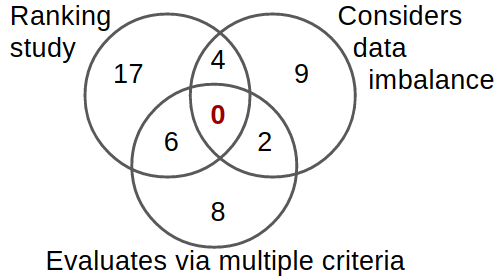
\includegraphics[width=2in]{venn.png}
\end{center}
\caption{Summary of papers from Table~\ref{tbl:survey2}.}
\label{fig:s2}
\vspace{-0.6cm}
\end{figure}
 
%\renewcommand\arraystretch{1.2}

% Accordingly, this paper is a ranking study that (a)~uses   multiple performance criteria to assess its classifiers; while (b)~fixing regions of the training
%  data with a weak signal  via synthetic data generation (using {\smb}, which is a self-tuning variant of {\sma}~\cite{chawla2002smote}). {\sma} is controlled by parameters which are normally set via ``expert judgement'' (a.k.a. guessing).
%  {\smb} uses a search-based SE technique called DE {\em differential evolution}~\cite{storn1997differential}) to automatically learn the best parameters for each data set. For more on {\smb}, see the next section.

% There are many studies done to find the best defect prediction performing model. Before 2007, it can be observed that almost every defect prediction study worked with 1 or 2 classification techniques evaluate on 1 or 2 measures. And almost none of the studies consider the effects of data imbalance. From Table~\ref{tbl:survey2} there has been ranking studies to find the best performing classifiers in about 16 out of 21 studies. Out of these 16, only 3 studied the effects of imbalance and among these 3 none studied for multiple evaluation goals.
% We highly agree to this given so many variations available in the data band there are so many classification techniques available like 

The key   observation to be made from  this 
survey is that, as shown in Figure~\ref{fig:s2}, no prior study in our sample satisfied  our definition of a ``good'' (see the ``0'' in the middle of the Venn diagram).
Accordingly, the rest of this
paper defines and executes a ``good'' ranking  study. A unique feature of our
ranking study is the use of an auto-tuning version of SMOTE.
 
 
\subsection{Handling Data Imbalance with SMOTE}
\label{sect:smote}

SMOTE handles class imbalance by changing the frequency of different classes of the training
data~\cite{chawla2002smote}. 
The algorithm's name is short for ``synthetic minority over-sampling technique''.
When applied to data, SMOTE sub-samples the majority class (i.e. deletes some examples)
while super-sampling the minority class
until
all classes have the same frequency.  In the case of software defect data,
the minority class is usually the  defective class.



Figure~\ref{fig:pseudocode} shows how SMOTE works. During super-sampling,
a member of the minority class finds $k$ nearest neighbors. It builds a fake member
of the minority class at some point in-between itself and one of its nearest
neighbors.  During that process, some distance function is required which, in Figure~\ref{fig:pseudocode}, is the {\em minkowski\_distance} function. 

\noindent
Note that SMOTE is controlled by these  parameters:
\bi
\item $k$ controls how many neighbors to use during over-sampling. Defaults to $k=5$.
\item $m$ is how many examples of each class are generated. Defaults to $m=50\%$ of the total training samples.
\item $r$ controls the distance function. The default is $r=2$;
i.e. use the  
standard Euclidean distance metric.
\ei

 
% Different data preprocessing has been proved
% to improve the performance of defect prediction models by
% Menzies et al.~\cite{menzies2007data}. Jiang et al.~\cite{jiang2008can} evaluate the impact of
% log transformation and discretization on the performance
% of defect prediction models, and report different modeling
% techniques ``prefer'' different transformation techniques. For
% instance, Naive Bayes achieves better performance on discretized
% data, while logistic regression achieves better performance
% for both. Peters et al.~\cite{peters2013better} propose different filters; and Li et al.~\cite{li2012sample} propose
% to use sampling. Nam et al.~\cite{nam2013transfer} transformed both
% training and testing data to the same latent feature space,
% and build models on the latent feature space. 
% %Too many variables in the datacan result in the ``curse of dimensionality''~\cite{friedman1997bias}.
% Feature Selection is a common method that can
% reduce features and sampling can balance the diversity of
% class instance numbers~\cite{yin2015empirical}, in turn improving the performance of defect prediction. In this paper we only tackle the class imbalance problem.


In the software analytics literature, there are contradictory findings on
the value of applying SMOTE for software defect prediction.
Van et al.~\cite{van2007experimental}, Pears et al.~\cite{pears2014synthetic} and Tan et al.~\cite{tan2015online} found SMOTE to be advantageous, while others, such as Pelayo et al.~\cite{pelayo2007applying} did not. 

Further, some researchers report that some learners respond better than others to standard SMOTE. Kamei et al.~\cite{kamei2007effects} evaluated the effects of SMOTE applied to  four fault-proneness models
(linear discriminant analysis, logistic regression, neural network and classification tree) by
using two module sets of industry legacy software. They reported that SMOTE improved the prediction performance of the linear and logistic models, but not neural network and classification tree models. Similar results, that the value of SMOTE was dependent on the learner,
was also reported by Van et al.~\cite{van2007experimental}.

\begin{figure}[!h]
\scriptsize
\begin{lstlisting}[mathescape,linewidth=8.2cm,frame=r,numbers=right]
  def SMOTE(k=2, m=50%, r=2):  # default settings
    while Majority > m do
      delete any majority item
    while Minority < m do
      add something_like(any minority item)
      
  def something_like(X0): 
    relevant = emptySet
    k1 = 0
    while(k1++ < 20 and size(found) < k)  {
       all = k1 nearest neighbors
       relevant += members of "all" of same class as X0 }
    Z = any of found
    Y = interpolate (X0, Z)
    return Y
    
  def minkowski_distance(a,b,r): 
    return $( \Sigma_i\ abs(a_i - b_i)^r)^{1/r}$
\end{lstlisting}
\caption{Pseudocode of SMOTE}
\label{fig:pseudocode}  
\end{figure}

\subsection{SMOTUNED = auto-tuning SMOTE}
\label{sect:smotuned}

One possible explanation for the variability in the {\sma} results is that the
default parameters of this algorithm are not suited to all data sets. To test this,
we designed {\smb}, which is an auto-tuning version of {\sma}. {\smb}
uses different control parameters for different data sets.


 
{\smb} uses DE (differential evolution~\cite{storn1997differential}) to explore the parameter space of
Table~\ref{tb:tuned}.  DE is an
optimizer useful for functions that may not be smooth or linear.  Vesterstrom et al.~\cite{Vesterstrom04} find   DE's optimizations to be  competitive with other optimizers like 
   particle swarm optimization or genetic algorithms.
   DEs have been used before for   parameter tuning~\cite{omran2005differential, chiha2012tuning,fu2016tuning,fu2017easy, agrawal2016wrong}) but this paper is  the first attempt to do
   DE-based class re-balancing.

\begin{figure}[!b]
\scriptsize
\begin{lstlisting}[mathescape,linewidth=8.2cm,frame=r,numbers=right]
  def DE( n=10, cf=0.3, f=0.7):  # default settings
    frontier = sets of guesses (n=10)
    best = frontier.1 # any value at all
    lives = 1
    while(lives$--$ > 0): 
      tmp = empty
      for i = 1 to $|$frontier$|$: # size of frontier
         old = frontier$_i$
         x,y,z = any three from frontier, picked at random
         new= copy(old)  
         for j = 1 to $|$new$|$: # for all attributes
           if rand() < cf    # at probability cf...
              new.j = $x.j + f*(z.j - y.j)$  # ...change item j
         # end for
         new  = new if better(new,old) else old
         tmp$_i$ = new 
         if better(new,best) then
            best = new
            lives++ # enable one more generation
         end                  
      # end for
      lives--
      frontier = tmp
    # end while
    return best
\end{lstlisting}
\caption{SMOTUNED uses DE (differential evolution).}
\label{fig:pseudo_DE}  
\end{figure}


As shown in Figure~\ref{fig:pseudo_DE}, DE evolves a \textit{frontier} of
candidates from an initial population. In the case of {\smb},
each  candidate is a randomly selected value for SMOTE's $k, m$ and $r$ parameters.
 To evolve the frontier, within each generation,
 DE compares each item to a {\em new} candidate generated
 by combining three other frontier items (and better {\em new} candidates replace
 older items). 
 To make that comparison, the {\em better} function on line 17 calls a learner on the training data using the proposed {\em new} parameters.
 When our DE  terminates, it returns the best {\em new} candidate ever seen in the entire run.
 
 While tuning, {\smb} explores 
the parameter ranges shown  in  Table~\ref{tb:tuned}. To define
the parameters, we found the range of used settings for {\sma} and distance functions
in the   SE and machine learning  literature.  Aggarawal et al.~\cite{aggarwal2001surprising}
argue that as data dimensionality, $r$ should shrink to some fraction less than one
(hence the bound of $r=0.1$ in Table~\ref{tb:tuned}. 

% \subsection{Importance of Tuning}
% \label{sect:tune}

% The previous section documented a strange difference of opinion
% about the value of SMOTE. One explanation for these differing results 
% is that SMOTE runs with different control parameters.
% The impact of tuning a learner's control parameters is well understood in the theoretical machine learning literature~\cite{bergstra2012random}.  When we tune a
% data miner for its performance, what we are really doing is changing how a learner applies its
% heuristics. This means tuned data miners use different heuristics, which means
% they ignore different possible models, which means they return different models;
% i.e. \textit{how} we learn changes \textit{what} we learn.

% Yet issues relating to
% tuning are poorly addressed in the software analytics literature. Fu et al.~\cite{fu2016tuning} surveyed a few of recent SE papers in the area
% of software defect prediction from static code attributes and found that SE
%   authors, with the exception of~\cite{tantithamthavorn2016automated} do not take steps to explore tunings. For example, Elish et
%   al.~\cite{elish2008predicting} compared support vector machines to other data
%   miners for the purposes of defect prediction. They tested different
%   ``off-the-shelf'' data miners on the same dataset, without adjusting the
%   parameters of each individual learner. Similar comparisons of data miners in SE,
% with no or minimal pre-tuning study, can be found in the work on Lessmann et al.~\cite{4527256}
% and, most recently, in Yang et al~\cite{Yang:2016}.  

% We choose to use DE after a literature search on search-based SE methods. DE is a method that optimizes a problem by iteratively trying to improve a candidate solution with regard to a given measure of quality.
% In the ast researchers have used many optimizers like: simulated
% annealing~\cite{feather2002converging, menzies2007business}; various genetic
% algorithms~\cite{goldberg1979complexity} augmented by techniques such as
% DE (differential evolution~\cite{storn1997differential}), tabu search and scatter
% search~\cite{glover1986general, beausoleil2006moss, molina2007sspmo,nebro2008abyss}; particle swarm optimization~\cite{pan2008particle}; numerous
% decomposition approaches that use heuristics to decompose the total space into
% small problems, then apply a response surface methods~\cite{krall2015gale, zuluaga2013active}.
% Of these, we use DE for two reasons. Firstly, it has been proven useful in prior SE tuning
% studies~\cite{fu2016tuning, agrawal2016wrong}. Secondly, our reading of the current literature is
% that there are many advocates for differential evolution.

% Fu et al.~\cite{fu2016tuning} showed that using DE to tune the parameters of software defect prediction learners results in large improvements, and the tuning was really simple. Similarly Agrawal et al.~\cite{agrawal2016wrong} tuned the parameters of LDA (Latent Dirichlet Allocation~\cite{blei2003latent}) and reports how tuning can provide better model stability. This shows how advantageous it is to tune the parameters of a data miner.


\begin{table}[!t]
    \begin{center}
\scriptsize
\begin{tabular}{c|c|c|p{3cm}} 
        \textbf{} & \textbf{Defaults} & \textbf{Tuning Range} & \\
          & \textbf{(used by  } & \textbf{(Explored  } &  \\  
        \textbf{Parameter} & \textbf{ SMOTE)} & \textbf{( SMOTUNED)} &  \textbf{Description} \\
          
          
        \hline
        $k$ & 5 & [1,20] & Number of neighbors \\ 
        \hline
       $m$ & 50\% & {50,100,200,400} & Number of synthetic examples to create. Expressed as a percent  of final training data. \\ 
        \hline
        $r$ & 2 & [0.1,5] & Power parameter for the Minkowski distance metric.\\
 
\end{tabular}
\end{center}
\caption{List of parameters tuned by this paper}
\label{tb:tuned}
\end{table}

\section{Experimental Design}
\label{sect:experiment}
 
This experiment  reports the effects of altering defect prediction
training
data   via {\smb} or {\sma} or not at all. 
 
 \begin{table}[!t]
\begin{center}
\begin{tabular}{r@{~}|r@{~}|r@{~}|r@{~}|r@{~}|r@{~}}
        \begin{tabular}[c]{@{}c@{}}\textbf{Version}\end{tabular} & \textbf{Dataset Name} & \textbf{Defect \%} & \textbf{Non-Defect \%} &\begin{tabular}[c]{@{}c@{}} \textbf{No. of} \\ \textbf{classes}\end{tabular}&\begin{tabular}[c]{@{}c@{}} \textbf{lines of} \\ \textbf{code} \end{tabular}\\ \hline
4.3 & jEdit & 2 & 98 & 492 & 202,363 \\ 
1.0 &   Camel & 4 & 96 & 339 & 33,721 \\  
6.0.3 &   Tomcat & 9 & 91 & 858 & 300,674\\ 
2.0 &   Ivy & 11 & 89 & 352 & 87,769 \\  
1.0 & Arcilook & 11.5 & 88.5 & 234 & 31,342\\ 
1.0 & Redaktor & 15 & 85 & 176 & 59,280 \\ 
1.7 & Apache Ant & 22 & 78 & 745 & 208,653 \\  
1.2 &   Synapse & 33.5 & 66.5 & 256 & 53,500 \\ 
1.6.1 &   Velocity & 34 & 66 & 229 & 57,012 \\\hline
  \multicolumn{4}{r|}{ total:} &    3,681&	1,034,314\\ 

\end{tabular}
\end{center}
\caption{Dataset statistics. Datasets are sorted from low percentage of defective class to high defective class.
Data comes from the SEACRAFT repository: http://tiny.cc/seacraft}.
\label{tb:dataset}
\vspace{-0.6cm}
\end{table}


\newcommand\fnote[1]{\captionsetup{font=small}\caption*{#1}}

\begin{figure*}[!b]
    \centering
    \begin{minipage}{.33\textwidth}
    \centering
    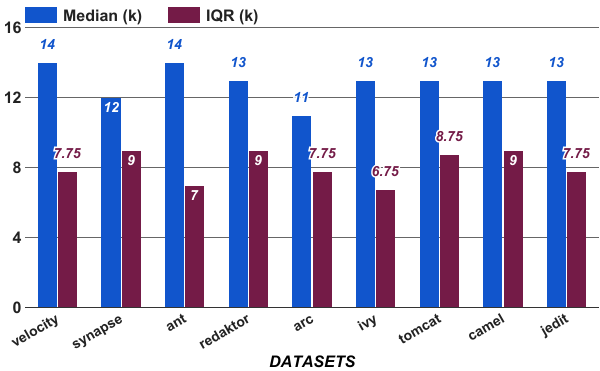
\includegraphics[width=.95\linewidth]{./fig/k.png}
        {\bf Figure~\ref{fig:para}a:} Tuned values for $k$\\ (default:  $k=5$).
    \end{minipage}~~%
    \begin{minipage}{.33\textwidth}
    \centering
        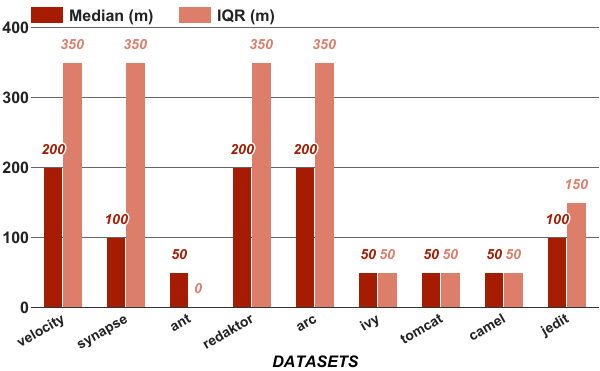
\includegraphics[width=.95\linewidth]{./fig/m.png}
        {\bf Figure~\ref{fig:para}b:} Tuned values for $m$\\ (default: $m=50\%$).
    \end{minipage}~~%
    \begin{minipage}{.33\textwidth}
    \centering
        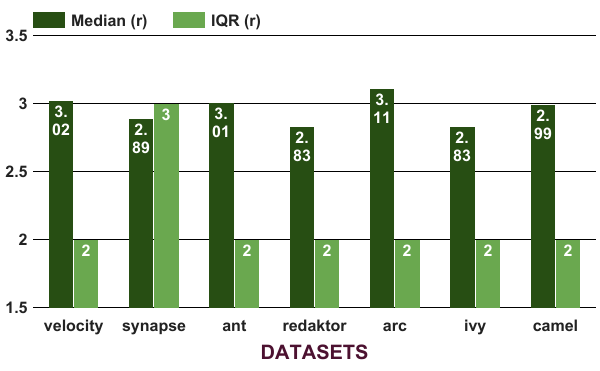
\includegraphics[width=.95\linewidth]{./fig/r.png}
        {\bf Figure~\ref{fig:para}c:} Tuned values for $r$\\ (default:  $r=2$).
    \end{minipage}
    \caption{Datasets vs Parameter Variation when optimized for recall and results reported on recall.
    ``Median'' denotes 50th percentile values seen in the 5*5 cross-validations and ``IQR'' shows the intra-quartile
    range; i.e. (75-25)th percentiles.}
    \label{fig:para}
\vspace{-0.4cm}
\end{figure*}



 
\begin{figure*}[!t]
\begin{minipage}{.5\linewidth}
\centering
        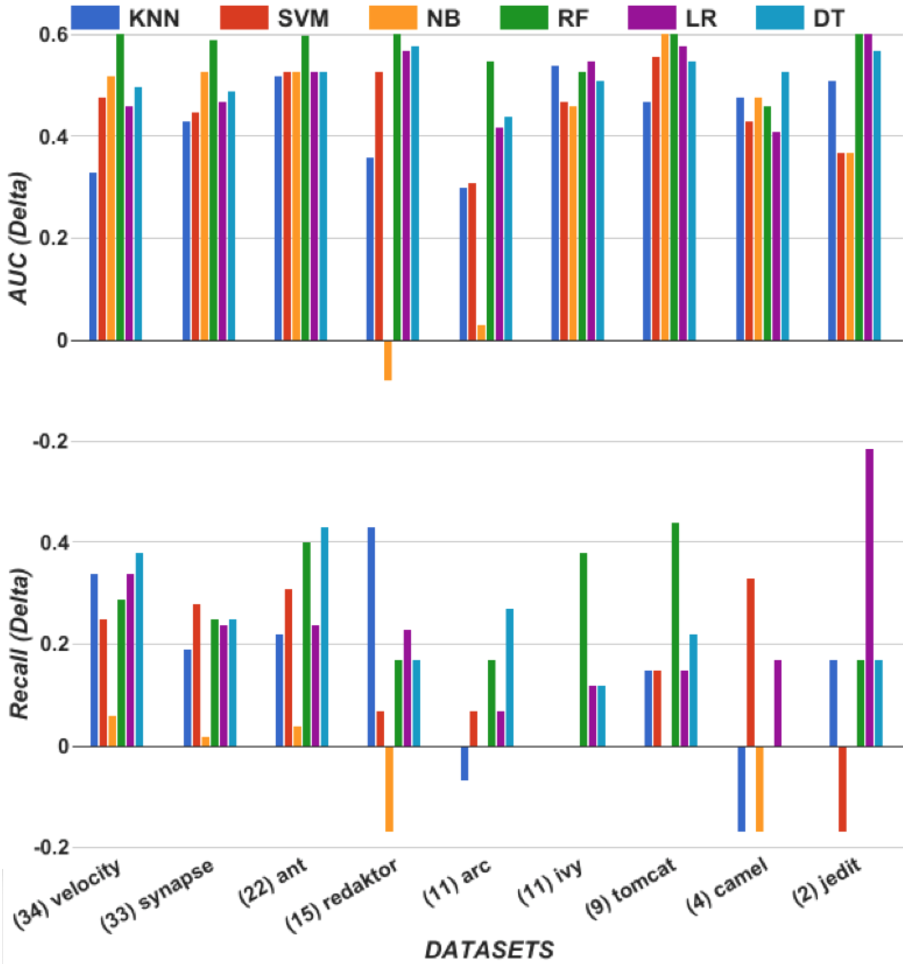
\includegraphics[width=.95\linewidth]{./fig/AUC_recall_tuned.png}
    \end{minipage}%
\begin{minipage}{.5\linewidth}
        \centering
        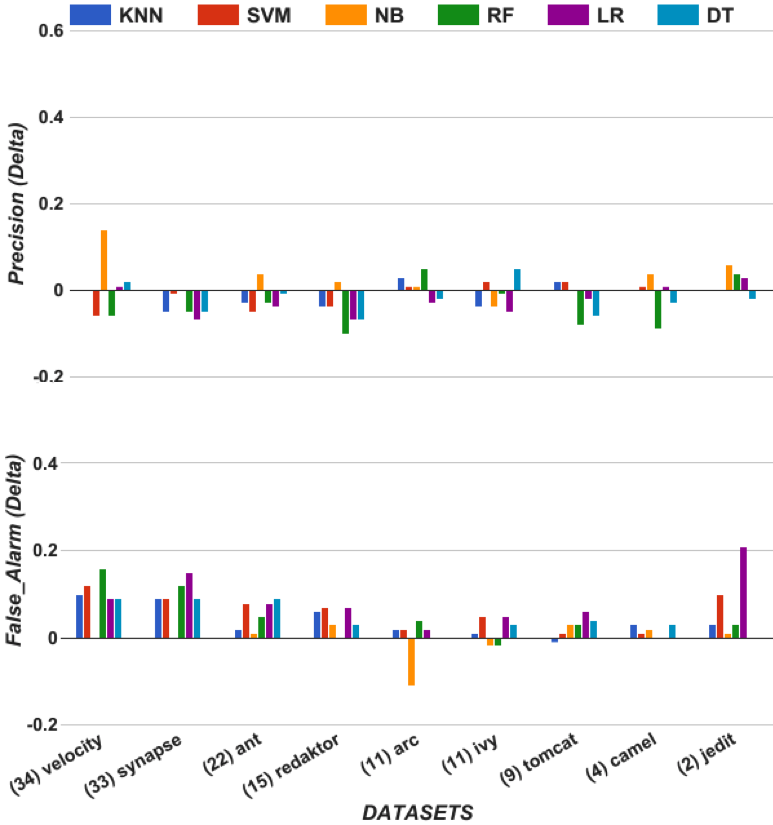
\includegraphics[width=.95\linewidth]{./fig/prec_pf_tuned.png}
    \end{minipage}%
    
    \caption{SMOTUNED improvement over SMOTE. \underline{Within}-Measure
    assessment (i.e. for each of these charts,
    optimize for performance measure $M_i$, then test for
    performance measure $M_i$). Note that for most charts
    {\em larger} values are {\em better}, but for false alarm,
    {\em smaller} values are {\em better}. Note that the corresponding percentage of minority class (in this case, defective class) is written beside each dataset.}
    \label{fig:tuned}
\vspace{-0.5cm}
\end{figure*}


Before proceeding 
we   stress the following methodological
principle.
To test the efficacy of any learner, it is important to
use test data whose class distributions match the real-world distributions.
Hence {\sma} (and {\smb}) should only
be applied to the training data {\em but
not to the test data}.



\subsection{Top-Level Loop}


Using some data $D_i \in D$, performance measure $M_i \in M$, and classifier $C_i \in C$,
this experiment conducts the 5*5 cross-validation study, defined below.
Our datasets  $D$ are shown in  Table~\ref{tb:dataset}. These are all open source
JAVA OO systems described in terms of the CK metrics described. 
Our performance measures $M$ were introduced in \tion{performance}
which includes   AUC, precision, recall, and the  false alarm. 
Our classifiers
 $C$  come from a  recent ICSE paper~\cite{ghotra2015revisiting}
and were listed in  Table~\ref{tbl:learners}.
For  implementations 
of these learners,
we used  the open source tool
Scikit-Learn~\cite{pedregosa2011scikit}.
Our  cross-validation study~\cite{refaeilzadeh2009cross} was defined as follows:
\be
\item We randomized the order of the data set $D_i$ set five times. This reduces the probability
that some random ordering of examples in the data will conflate our results.
\item Each time, we divided the data $D_i$ into five bins;
\item For each bin (the test), we trained on four bins (the rest) and then tested
on the test bin as follows:
\be
\item
Important point: {\em we only {\sma} the training data,  leaving
the  testing data unchanged}.
\item
The  training set is pre-filtered using either No-SMOTE (i.e. do nothing) or  {\sma} or {\smb}.  
\item
When using {\smb}, DE is  run to  improve
the performance measure $M_i$ seen when the classifier $C_i$ was applied to the training data.
Important note: {\em when tuning {\sma}, this rig \underline{{\em never}} uses test data}.
\item
After pre-filtering, a classifier $C_i$  learns a predictor.
\item
The model is applied to the test data to collect performance measure $M_i$. 
\item 
We print the {\em performance delta} between this $M_i$ and another  $M_i$
generated from applying $C_i$ to the raw data $D_i$ (i.e. compared to learning
without any filtering).
\ee
\ee


   
   
Note that the above rig tunes {\sma}, but not the control parameters of the classifiers.
We do this since, in this paper,  we aim to document the   benefits of tuning {\sma} since as shown below, they are very large indeed. Also, it would be  pragmatically very useful if we can show that a single algorithm ({\smb})  improves the performance of defect prediction. This would allow
subsequent work to focus on the task of optimizing  {\smb} (which would be a far easier
task than optimizing the tuning of a wide-range of classifiers). 
 

\subsection{Within- vs Cross-Measure Assessment}
\label{sect:wcm}
We call the above rig as the {\em within-measure assessment rig} since it is  biased in its evaluation measures. Specifically,  in this rig,
when {\smb} is optimized for (e.g.) AUC, we do not explore the effects on (e.g.) the false alarm. This is less than ideal
since it is known that our performance measures are inter-connected via the Zhang equation~\cite{zhang2007comments}. Hence, increasing (e.g.) recall might potentially have the adverse
effect of  driving up (e.g) the false alarm rate. 
To avoid this problem, we also apply the following {\em cross-measure assessment rig}.
At the conclusion of the {\em within-measure assessment rig}, we will observe  that the AUC performance measure will show the largest improvements. Using that best performer, we will re-apply steps 1,2,3 abcdef (listed above) but this time:
\bi
\item In step 3c, we will tell {\smb} to optimize for AUC;
\item In step 3e, 3f we will collect the performance delta on AUC as well as precision, recall,
and false alarm.
\ei
In this approach, steps 3e and 3f collect the information required   to check if succeeding according to one performance criteria results in damage to another.


\subsection{Statistical Analysis}

When comparing the results of {\smb} to other
treatments, we use a statistical
significance test and an effect size test.
Significance test are usefully for detecting if two populations
differ merely by random noise. 
Also, effect sizes are useful for checking that two populations differ by more than just a trivial amount.

For the significance test,  we use the 
     Scott-Knott procedure  recommended  recently in TSE'13~\cite{mittas13} and at ICSE'15~\cite{ghotra2015revisiting}. This
     technique recursively bi-clusters a sorted
    set of numbers. If any two clusters are statistically indistinguishable, Scott-Knott
    reports them both as one group.
    Scott-Knott first looks for a break in the sequence that maximizes the expected
    values in the difference in the means before and after the break.
    More specifically,  it  splits $l$ values into sub-lists $m$ and $n$ in order to maximize the expected value of differences  in the observed performances before and after divisions. E.g. for lists $l,m$ and $n$ of size $ls,ms$ and $ns$ where $l=m\cup n$, Scott-Knott divides the sequence at the break that maximizes:
     \[E(\Delta)=ms/ls*abs(m.\mu - l.\mu)^2 + ns/ls*abs(n.\mu - l.\mu)^2\]
Scott-Knott then applies some statistical hypothesis test $H$ to check if $m$ and $n$ are significantly different. If so, Scott-Knott then recurses on each division.
    For this study, our hypothesis test $H$ was a conjunction of the A12 effect size test (endorsed by
    \cite{arcuri11})  and non-parametric bootstrap sampling \cite{efron94}; i.e. our Scott-Knott divided the data if {\em both}
    bootstrapping and an effect size test agreed that the division was statistically significant (99\% confidence) and not a ``small'' effect ($A12 \ge 0.6$).



% \subsection{\textbf{Preprocessing and Classifiers}}
% \label{sect:classes}
%  We ignored  string columns in the data and assumed that the last column in the dataset is always the target class. Originally, the target class contains number of defects, which we converted to binary, i.e if target class has defect then it represents 1 otherwise it denotes 0. The code assumes user has preprocessed the data before passing it to the learners. 

% We used six classifiers which are mentioned in the baseline paper~\cite{ghotra2015revisiting} using the default
% parameters suggested by Ghotra et al. Those classifiers are Support Vector Machines (SVM - Linear Kernel), Linear Regression (LR), Naive Bayes (NB), K Nearest Neighbors (KNN - $K=8$), Decision Trees (DT - CART, Split Criteria=Entropy) and Random Forests (RF - Split Criteria=Entropy). Most of these implementations are provided in Scikit-Learn~\cite{pedregosa2011scikit} and available open source. There are some tie breaking instances during training. For instance, in K-NN, default $K$ used is an even number and we are randomly tie breaking to pick any 8th neighbor.

% \bi
%  \item \textbf{Support Vector Machines (SVM - Linear Kernel)} are supervised learning models with associated learning algorithms that analyze data used for classification and regression analysis. Given a set of training examples, each marked as belonging to one or the other of two categories, an SVM training algorithm builds a model that assigns new examples to one category or the other, making it a non-probabilistic binary linear classifier.
%  \item \textbf{Linear Regression (LR)} is an approach for modeling the relationship between a scalar dependent variable $y$ and one or more explanatory variables (or independent variables) denoted $x$.
%  \item \textbf{Naive Bayes (NB)} classifiers are a family of simple probabilistic classifiers based on applying Bayes theorem with strong (naive) independence assumptions between the features.
%  \item \textbf{K Nearest Neighbors (KNN - $K=8$)} is a non-parametric method used for classification and regression. In both cases, the input consists of the $k$ closest training examples in the feature space. Since $k$ is even, for tie breaking a random result is selected.
%  \item \textbf{Decision Trees (DT - CART, Split Criteria=Entropy)} are a decision support tool that use a tree-like graph or model of decisions and their possible consequences, including chance event outcomes, resource costs, and utility. It is one way to display an algorithm.
%  \item \textbf{Random Forests (RF - Split Criteria=Entropy)} are an ensemble learning method for classification, regression and other tasks, that operate by constructing a multitude of decision trees at training time and outputting the class that is the mode of the classes (classification) or mean prediction (regression) of the individual trees. 
% \ei

% Similar Ghotra et al.~\cite{ghotra2015revisiting}, we used $k=8$ for $k$ Nearest Neighbours. Also for Decision trees and Random Forest we used Entropy as split criteria. 

 





% \renewcommand{\algorithmicrequire}{\textbf{Input:}}
% \renewcommand{\algorithmicensure}{\textbf{Output:}}
% \begin{algorithm}
%  \scriptsize
%     \begin{algorithmic}[1]
%     \Require $np=10$, $f=0.7$, $cr=0.3$, $iter=3$, Goal $\in$ Finding maximum/minimum score
%     \Ensure $Score, final\_generation$
%     \Function{DE}{$np,f,cr,iter, Goal$}
%         \State  $Cur\_Gen \leftarrow \emptyset$
%         \State $Population \leftarrow $InitializePopulation(np)
%         \For{$i = 0$ to $np-1$}
%             \State $Cur\_Gen$.add($Population$[i],score)
%         \EndFor
%         \For{$i = 0$ to $iter$}
%             \State $NewGeneration \leftarrow \emptyset$
%             \For{$j = 0$ to $np-1$}
%                 \State $S_i \leftarrow $Extrapolate($Population$[j],Population,cr,f,np)
%                 \If{score($S_i$) $\geq$ $Cur\_Gen$[j][1]}
%                     \State $NewGeneration$.add($S_i$,score($S_i$))
%                 \Else
%                     \State $NewGeneration$.add($Cur\_Gen$[j])
%                 \EndIf
            
%             \EndFor
%             \State  $Cur\_Gen \leftarrow NewGeneration$
%         \EndFor
%         \State $Score \leftarrow$ GetBestSolution($Cur\_Gen$)
%         \State  $final\_generation \leftarrow Cur\_Gen$
%         \State \textbf{return} $Score, final\_generation$
%     \EndFunction

%     \Function{Extrapolate}{$old, pop, cr, f,np$}
%         \State $a,b,c \leftarrow threeOthers$(pop, old)
%         \State $newf \leftarrow \emptyset$
%         \For{$i = 0$ to $np-1$}
%             \If{$cr \leq$ random()}
%                 \State $newf$.add($old[i]$)
%             \Else
%                 \If{typeof($old$[i])$ ==$ bool }
%                     \State $newf$.add(not $old[i]$)
%                 \Else 
%                     \State $newf$.add(trim(i,($a$[i]+$f\ast$($b$[i] $-$ $c$[i]))))
%                 \EndIf
%             \EndIf
%         \EndFor
%         \State \textbf{return} $newf$ 
%     \EndFunction
%     \caption{Pseudocode for DE with a constant number of iterations}
%     \end{algorithmic}
% \end{algorithm}


% The loop invariant of DE is that, after the i-th iteration$^7$, the \textit{Population}
% contains examples that are better than at least one other candidate.
% As the looping progresses, the \textit{Population} is full of increasingly more valuable solutions
% which, in turn, also improve the candidates, which are extrapolated from the Population.
% Hence, Vesterstrom et al.~\cite{vesterstrom2004comparative} found DE to be
% competitive with particle swarm optimization and other GAs.


% \begin{figure*}[!t]
% \begin{minipage}{.5\linewidth}
% \centering
%         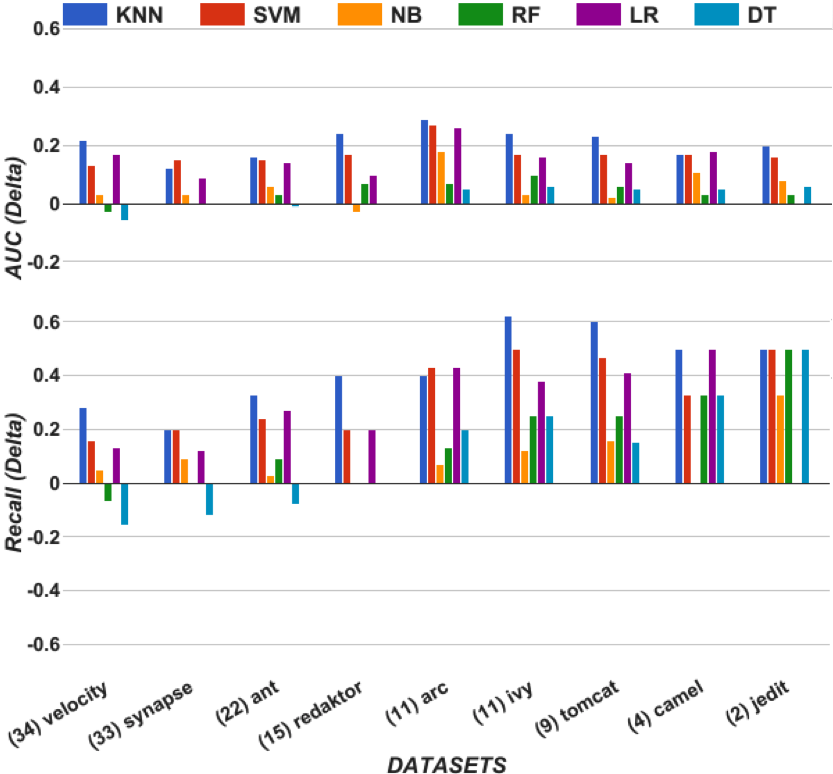
\includegraphics[width=.95\linewidth]{./fig/AUC_recall_untuned.png}
%     \end{minipage}%
% \begin{minipage}{.5\linewidth}
%         \centering
%         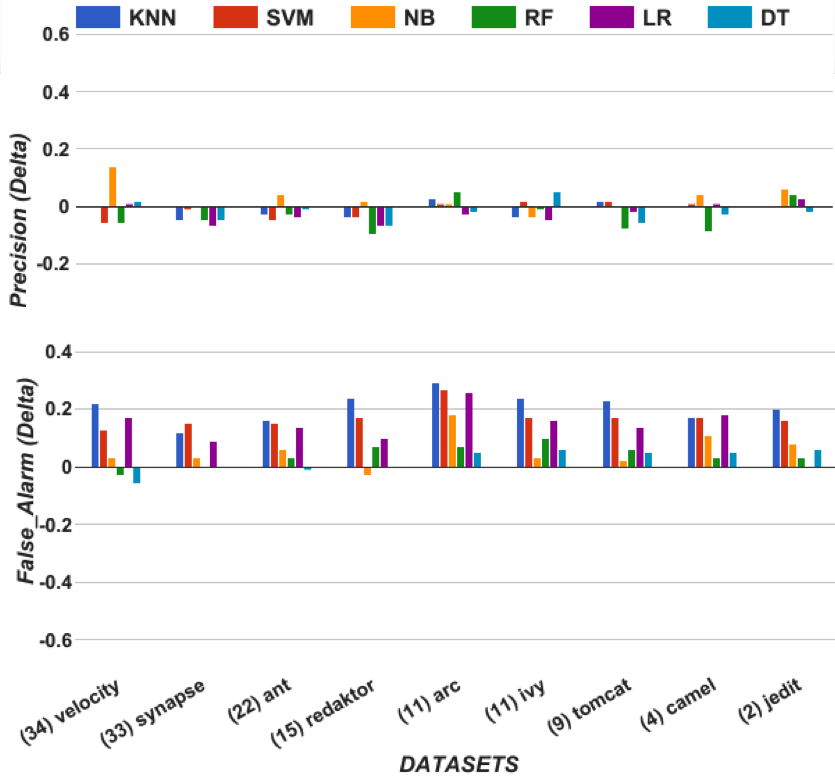
\includegraphics[width=.95\linewidth]{./fig/prec_pf_untuned.png}
%     \end{minipage}%
%     \caption{SMOTE improvement over No-SMOTE. Legends represent the classifiers mentioned in \tion{classes}}
%     \vspace{-11pt}
%     \fnote{For subfigures (AUC, Recall and Precision): larger y-values are {\em better}, if the y-value goes {\em negative}, then the corresponding learner trained on SMOTE data performs {\em worse} than learner learnt on raw data. For false alarms, the plot must be interpreted differently: larger y-values are {\em worse}, if the y-value goes {\em positive}, then the corresponding learner trained on SMOTE data performs {\em worse} than learner learnt on raw data. The corresponding percentage of minority class (in this case, defective class) is written beside each dataset.}
%     \label{fig:untuned}
% \end{figure*}
 
 
% \newcommand\fnote[1]{\captionsetup{font=small}\caption*{#1}}

% \begin{figure*}[!t]
% \begin{minipage}{.5\linewidth}
% \centering
%         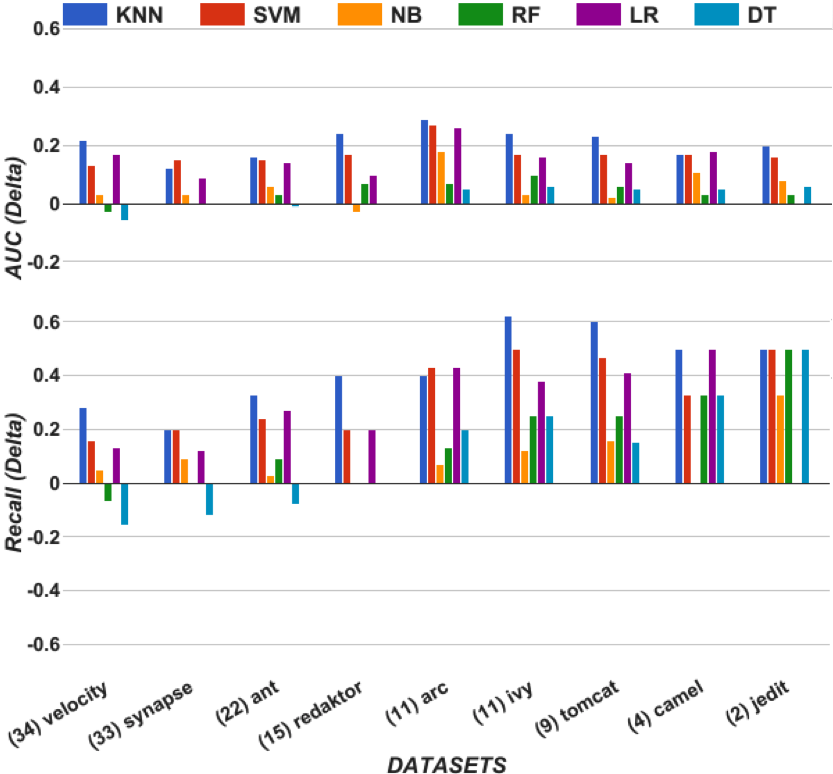
\includegraphics[width=.95\linewidth]{./fig/AUC_recall_untuned.png}
%     \end{minipage}%
% \begin{minipage}{.5\linewidth}
%         \centering
%         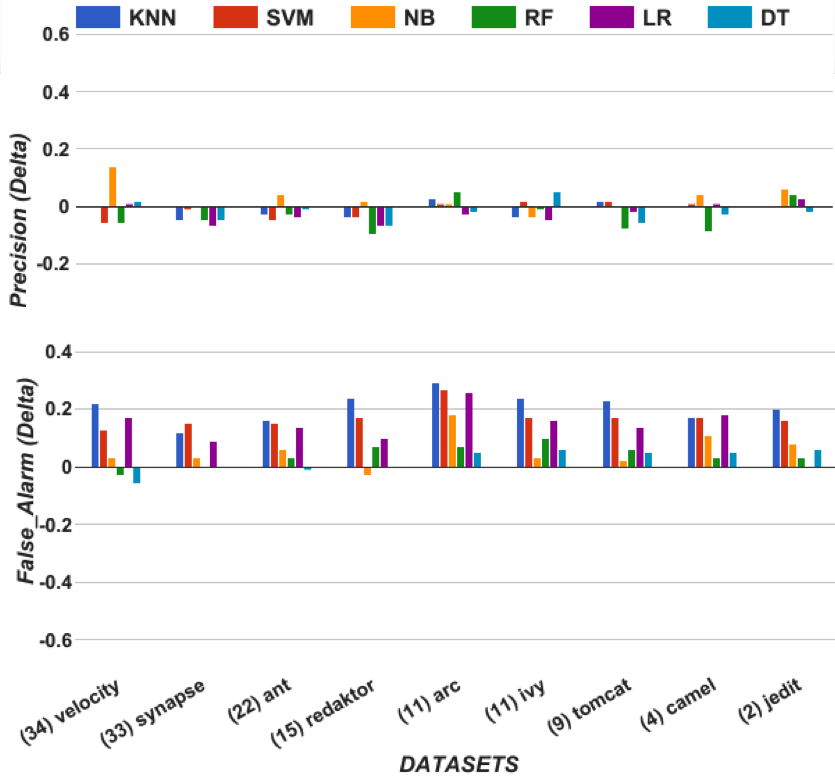
\includegraphics[width=.95\linewidth]{./fig/prec_pf_untuned.png}
%     \end{minipage}%
%     \caption{SMOTE improvement over No-SMOTE. Legends represent the classifiers mentioned in \tion{classes}}
%     \vspace{-11pt}
%     \fnote{For subfigures (AUC, Recall and Precision): larger y-values are {\em better}, if the y-value goes {\em negative}, then the corresponding learner trained on SMOTE data performs {\em worse} than learner learnt on raw data. For false alarms, the plot must be interpreted differently: larger y-values are {\em worse}, if the y-value goes {\em positive}, then the corresponding learner trained on SMOTE data performs {\em worse} than learner learnt on raw data. The corresponding percentage of minority class (in this case, defective class) is written beside each dataset.}
%     \label{fig:untuned}
% \end{figure*}

 
   

\section{Results}
\label{sect:results}

Our results are organized around the three
research questions introduced in \tion{intro} of this paper.

 \subsection{{\bf RQ1}: Are the default ``off-the-shelf'' parameters for SMOTE appropriate for all
 data sets?}
 
 
 As discussed above, the default parameters for
 {\sma} are $k,\ m$ and $r = 5,\ 50\%$ and $2$.
  Figure~\ref{fig:para} shows the range of parameters
 found by {\smb} across  nine data sets for the 25 repeats of our cross-validation procedure.
 All the results in this figure are {\em within-measure assessment} results; i.e.
 here, we {\smb}  on a particular performance measure and then we only collect performance for that performance measure on the test set.
 
 
 In  Figure~\ref{fig:para}, the {\em median} is the 50th percentile
 value and {\em IQR} is the (75-25)th percentile
 (IQR is a non-parametric analogue of variance).
 As can be seen in Figure~\ref{fig:para}, most of the learned parameter are far from the default values:
 \bi
 \item 
 Median $k$ value was never less than 11;
 \item
 Median $m$ value differs according to each dataset and quite far from the actual;
 \item
 The $r$ value used in the distance function was never 2. Rather, it was usually 3.
 \ei
 Hence,  our answer to {\bf RQ1} is ``no'': the use of off-the-shelf {\sma} should be deprecated. 
 
 Before moving on to {\bf RQ2}, we note that many of the settings in Figure~\ref{fig:para} are very similar; for example, median values of $k=13$ and $r=3$ seems to be a common
result.  Nevertheless, we do {\em not} recommend replacing
the defaults on regular {\sma} with the median values
of Figure~\ref{fig:para}. In that figure, many of the  IQR bars are
very large (IQR=intra-quartile range = denotes the
75th-25th percentile). Clearly, SMOTUNED's decisions vary dramatically
depending on what data  is being processed.  Accordingly,
we strongly recommend that {\smb} be applied to each new data set.



\begin{figure*}[!t]
\begin{minipage}{.5\linewidth}
\centering
        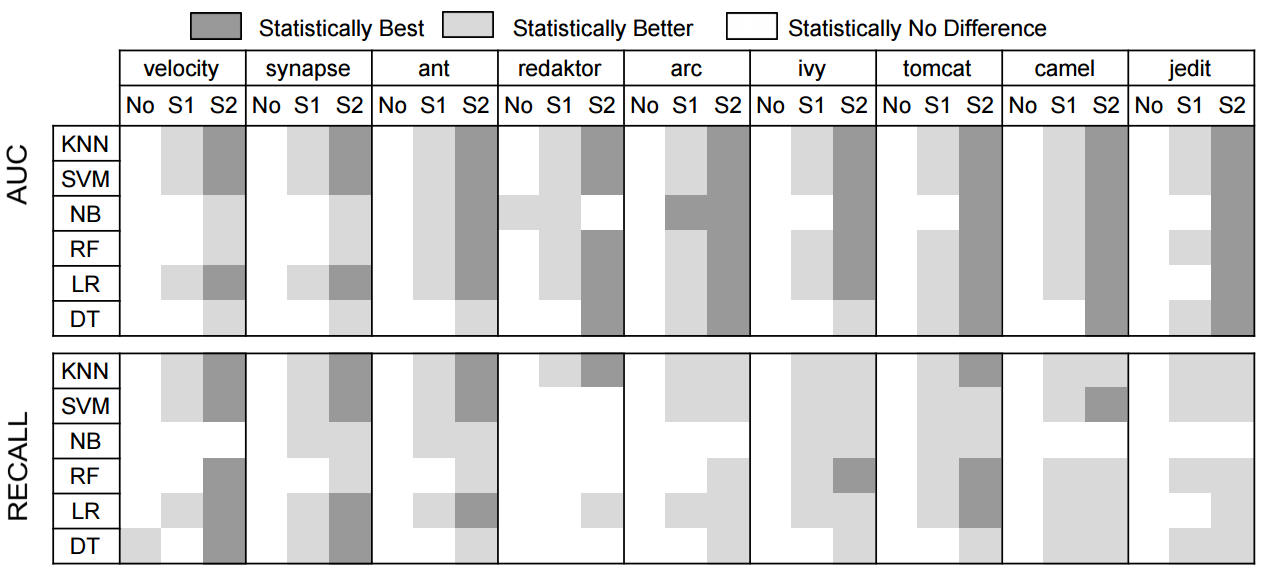
\includegraphics[width=1\linewidth]{./fig/AUC_recall.png}
            \end{minipage}%
\begin{minipage}{.5\linewidth}
        \centering
        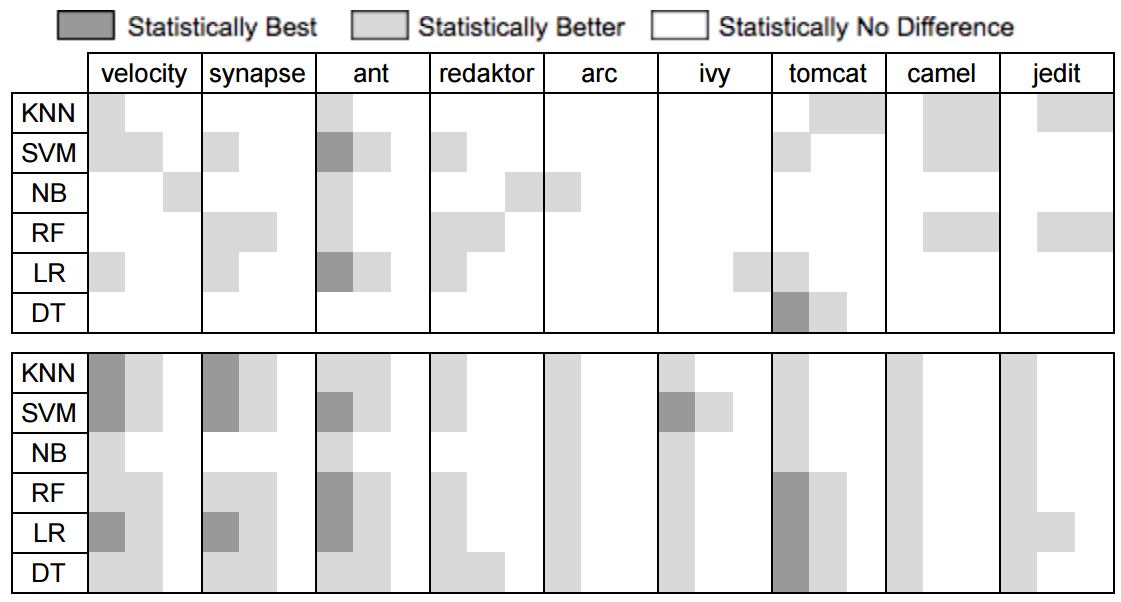
\includegraphics[width=1\linewidth]{./fig/prec_pf.png}
    \end{minipage}%
    \caption{Scott Knott analysis of No-SMOTE, SMOTE and SMOTUNED. The column headers are denoted as No for No-SMOTE, S1 for SMOTE and S2 for SMOTUNED. $(\ast)$ Mark represents the best learner combined with its techniques.}
    \label{fig:stats}
\vspace{-0.5cm}
\end{figure*}


\subsection {{\bf RQ2}: Is there any benefit in tuning the default parameters of SMOTE for each new data set?}

Figure~\ref{fig:tuned} shows the performance delta of the {\em within-measure assessment rig}.
Recall that when this rig applies {\smb}, it optimizes for performance measure
\[M_i \in \{ 
\mathit{recall},
\ \mathit{precision}, 
\ \mathit{false\; alarm},
\ \mathit{AUC}
\}
\]
after which it uses the {\em same} performance measure
$M_i$ when processing the test data.
As shown in Figure~\ref{fig:tuned}, 
{\smb} achieves large AUC and recall improvements
without
 damaging precision and  with only minimal changes
 to false alarm. A special note should be taken of the AUC improvements- these are the largest improvements
 we have yet seen, for any prior treatment of defect prediction data.

Figure~\ref{fig:stats} offers a statistical analysis
of different results achieved
after applying our three data pre-filtering methods:
\bi
\item  {\em NO} = do nothing;
\item {\em S1} = use default {\sma};
\item {\em S2} = use {\smb}.
\ei
For any learner, there are three such treatments and {\em darker} the cell, {\em better} the performance. 
In that figure, cells with the same color are
either not statistically significantly different or
are different only via a {\em small effect}
(as judged by the statistical methods described above).

As to what combination of pre-filter+learner works better for any data set, that is marked by a ``*''. Since we have three pre-filtering methods and six learners, there is one   ``*'' per 18 cells in Figure~\ref{fig:stats}.

In the  AUC and recall results,  the best ``*'' cell always appears in the S2={\smb} column. 
That is, for those two performance measures,  {\smb} is always
used by the best combination of pre-filter+learner .

As to precision  results,  at first glance, the  results in Figure~\ref{fig:stats} look bad for {\smb} since, less than half the times, 
the best ``*''  happens  in S2={\smb} column.
 But recall from Figure~\ref{fig:tuned} that the absolute size of the precision deltas is very small.  Hence, even though {\smb} ``losses'' in this statistical analysis, the pragmatic impact of that result  is  negligible.
 
As to the false alarm results of Figure~\ref{fig:stats}, as discussed above in \tion{performance}, the cost of increased recall is to also increase
the false alarm rate. For example, the greatest \textit{increase} in recall was 0.58 seen in the {\em jEdit} results. This increase comes at a cost
of \textit{increasing} the false alarm rate by 0.20. Apart from this one large outlier, the overall pattern is that the recall improvements range from +0.18 to +0.42 (median to max)
and these come at the cost of much smaller false alarm \textit{increase} of 0.07 to 0.16 (median to max). 
 
In summary, the answer to {\bf RQ2} is that our  AUC and recall results strongly endorse the  use of {\smb}
while the precision and false alarm rates
show there is little harm in using {\smb}.

Before moving to the next research question, we note that these
 results offer an interesting insight on prior ranking studies that rank some learners
as ``better'' than another.
Recall from Table~\ref{tbl:learners} that prior studies have offered an approximate ranking for different learners; specifically:
\[
(\mathit{RF},\mathit{LR}) > (\mathit{KNN},\mathit{NB}) > (\mathit{DT}) > (\mathit{SVM})
\]
If we count how often our learners perform
best in the AUC and recall results of Figure~\ref{fig:stats} (i.e. how many times they were marked with ``*'') then, at first
glance, it would seem that Figure~\ref{fig:stats} is recommending very nearly the same
learners as ``best'' for defect prediction as   Table~\ref{tbl:learners}:
\[
\begin{array}{c}
(\mathit{RF}=7) > (\mathit{LR}=5) > (\mathit{KNN}=4) >\\
(\mathit{SVM}=2) > (\mathit{NB}=0, \mathit{DT}=0)
\end{array}
\]
Here, we do not count  the precision and false alarm counts since, as discussed above, the size
of that delta is so small to be pragmatically negligible (particularly when compared to the AUC+recall effects).

The key point here is that there are 18 experiments in the left-hand-side of Figure~\ref{fig:stats}. That is,
even though RF (random forests) has the highest  ``best'' scores, it still defeated in \mbox{$(18-7)/18=61\%$}
experiments. This means that we must doubt the conclusions of prior ranking studies like 
 Table~\ref{tbl:learners} since we find that no   learner was  consistently  ``best''  across most of our experiments.
On the other hand, 
  {\smb} was  consistently  used  by  whatever  learner  was  found  to  be ``best'' (in recall and AUC). 
Hence, we conclude from the {\b RQ2} results that  prior ranking study results (that only assessed different learners) have missed a much more general effect about the benefits of data pre-processing.
To say that another way, ``better data'' might be better than ``better data miners''.

As a last note about the {\bf RQ2} results, we note that they offer a new insight into
the true value of methods of {\sma}.
When we drew the plots of  Figure~\ref{fig:tuned}, we deliberately ordered
the x-axis data sets according to their imbalance:
\bi
\item
The data sets with the {\em highest} ratio of defects (Velocity and Synapse) are shown on the left-hand side of each plot in Figure~\ref{fig:tuned}.
\item
While the data sets with the {\em lowest} ratio of defects (jEdiot and Camel) are shown on the right-hand side.
\ei
Given that ordering of the x-axis, then if  repairing class imbalance  improved predictor performance, then 
we should see most improvements on the right hand side of the  Figure~\ref{fig:tuned} plots.
This is not the case (and effect size tests confirm that visual impression).
Hence, we conjecture that the   real value of {\sma} (and {\smb}) is not fixing the class imbalance, rather, SMOTE's
value might be in {\em amplifying} the data's signal in spare regions of the data (by filling
in those regions with synthetic examples extrapolated from the local region). 


\subsection{{\bf RQ3:} In  terms  of  runtimes,  is  the  cost  of  running  {\smb} worth the performance improvement?}

Figure \ref{runtime} shows the mean runtimes
for running a 5*5 cross-validation study for six learners for each data set.
These runtimes were collected from one machine running CENTOS7, with 16 cores.
Note that they do not increase monotonically with the size of the data sets since:
\bi
\item Our version of {\sma} uses ball trees to optimize the nearest neighbor calculations. Hence, the runtime of that algorithm is dominated by the internal topology of the data sets rather than the number of classes.
\item
As shown in 
Figure~\ref{fig:pseudocode} (lines 9-12),
{\smb} explores the local space until it finds $k$ neighbors of the same class. This can take a variable amount of time to terminate.
\ei
As might be expected,  {\smb} is an order of magnitude slower than {\sma} since
it has to run {\sma} many times to assess different parameter settings.
That said, in absolute term, those runtimes are not excessively slow.
{\smb} usual terminates in under two minutes and never more than half an hour.
% Figure~\ref{runtime} by 5*5*6=150, we see that even for our slowest data sets (tomcat), one run
% of SMOTUNED terminated in 34284/150=228 seconds (on an average), which is less than four minutes.
Hence, in  our opinion, we answer {\bf RQ3} as ``yes'' since the   performance increases
seen in Figure~\ref{fig:tuned} more than compensate for the extra CPU required for {\smb}.
 

\begin{figure}[!t]
  \captionsetup{justification=centering}
                                                   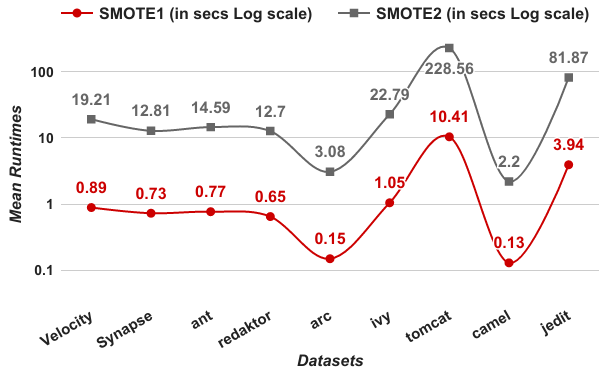
\includegraphics[width=\linewidth]{./fig/runtimes.png}
  \caption{Datasets vs Runtimes. Note that the numbers
  shown here are the mean times seen across 25 repeats of a 5*5 cross-validation study.
  %running six learners through a 5*5 cross-validation. Hence, for mean
  %runtimes for one learner, {\em divide} these numbers by 6*5*5=150.
  }
  \label{runtime}
\vspace{-0.6cm}
\end{figure}

\begin{figure*}[!htbp]
\begin{minipage}{.5\linewidth}
\centering
        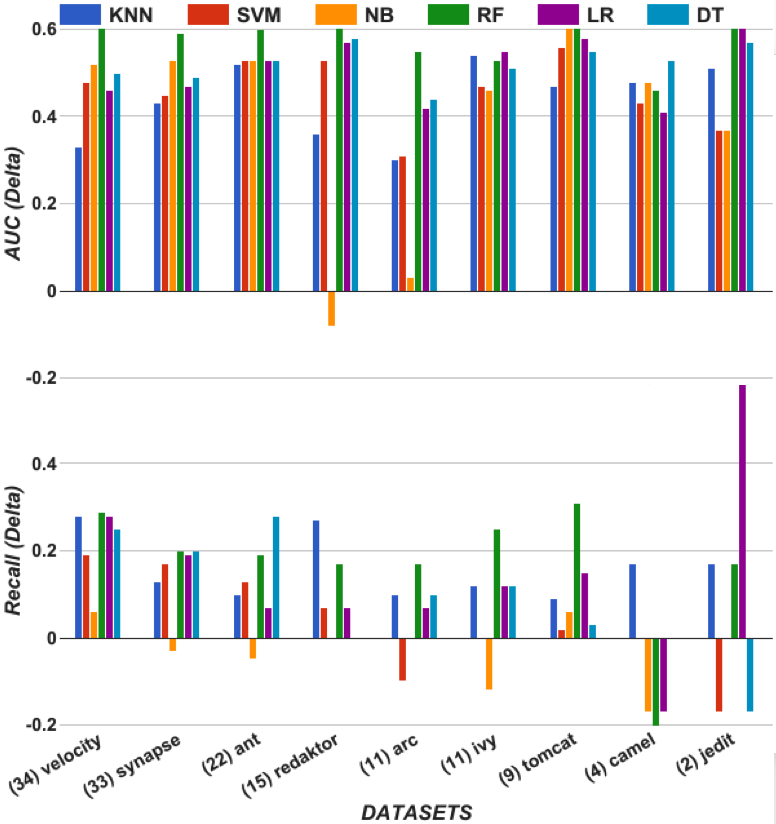
\includegraphics[width=.95\linewidth]{./fig/AUC_auc1.png}
    \end{minipage}%
\begin{minipage}{.5\linewidth}
        \centering
        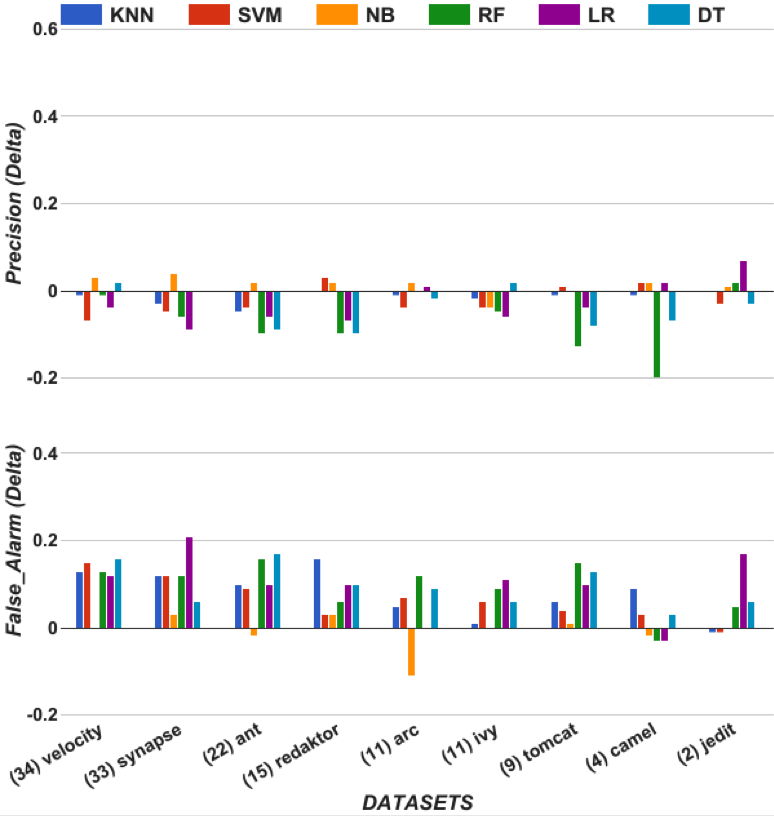
\includegraphics[width=.95\linewidth]{./fig/AUC_prec.png}
    \end{minipage}%
    
    \caption{ SMOTUNED improvement over SMOTE. 
    \underline{{\bf Cross}}-Measure
    assessment (i.e. for each of these charts,
    optimize for \underline{{\bf AUC}}, then test for
    performance measure $M_i$).  Same format as
    Figure~\ref{fig:tuned}.}
    \label{fig:auc22}
\vspace{-0.6cm}
\end{figure*} 
\section{Threats to Validity}
\label{sect:validity}

As with any empirical study, biases can affect the final
results. Therefore, any conclusions made from this work must consider the following issues in mind.

\textbf{\textit{Order bias}}: With each dataset how data samples are distributed in training and testing set is completely random. Though there could be times when all good samples are binned into training and testing set. To mitigate this order bias, we run
the experiment 25 times by randomly changing the order of the data samples each time.

\textbf{\textit{Sampling bias}} threatens any classification experiment; i.e., what matters there may not be true here. For example, the datasets used here comes from the SEACRAFT repository and were supplied by one individual. These datasets have used in various case studies by various researchers~\cite{he2012investigation,peters2013better,peters2013balancing,turhan2013empirical}; i.e. our results are not more biased that many other studies in this arena.
That said, our nine open-source datasets   are mostly from Apache. Hence
it is an open issue if our results hold for
 proprietary projects and open source projects from other sources.

% \textbf{\textit{Learner bias}}: For building the defect predictors in this
% study, we selected each learner with default parameters like k=8 in $k$-NN, entropy as split criteria in RF, and DT. The above predefined parameters have been used in the conclusions made by other studies~\cite{ghotra2015revisiting,tantithamthavorn2016automated}. 

\textbf{\textit{Evaluation bias}}: In terms of evaluation bias,
our study is far less biased than many other ranking studies.  As shown by our sample of
22 ranking studies in
Table~\ref{tbl:survey2}, 19/22 of those prior studies used {\em fewer} evaluation criteria
than the four reported here (AUC, recall, precision and false alarm). 

That said, there is another more subtle evaluation bias in  Figure~\ref{fig:tuned}. Note that the four plots of that figure are four {\em different} runs of our  {\em within-measure assessment rig}
(defined in \tion{wcm}). Hence, it is reasonable to check what happens when (a)~one
evaluation criteria is used control {\smb}, and (b)~the results are assessed
using all four evaluation criteria. 
Figure~\ref{fig:auc22} shows the results of such a {\em cross-measure assessment rig} where AUC was used to control {\smb}. We note that:
\bi
\item
The results in this figure are very similar to   Figure~\ref{fig:tuned}; e.g. the precision deltas aver usually tiny, and false alarm increases are usually smaller than the associated recall improvements. 
\item
But there are some larger improvements in Figure~\ref{fig:tuned}
than Figure~\ref{fig:auc22}.
\ei
Hence, we recommend cross-measure assessment only if CPU is critically restricted. Otherwise, we think {\smb} should be controlled by whatever is the downstream evaluation criteria
(as done in the within-measure assessment rig of Figure~\ref{fig:tuned}.)

% \begin{figure}[!htbp]
% \begin{minipage}{\linewidth}
% \centering
%         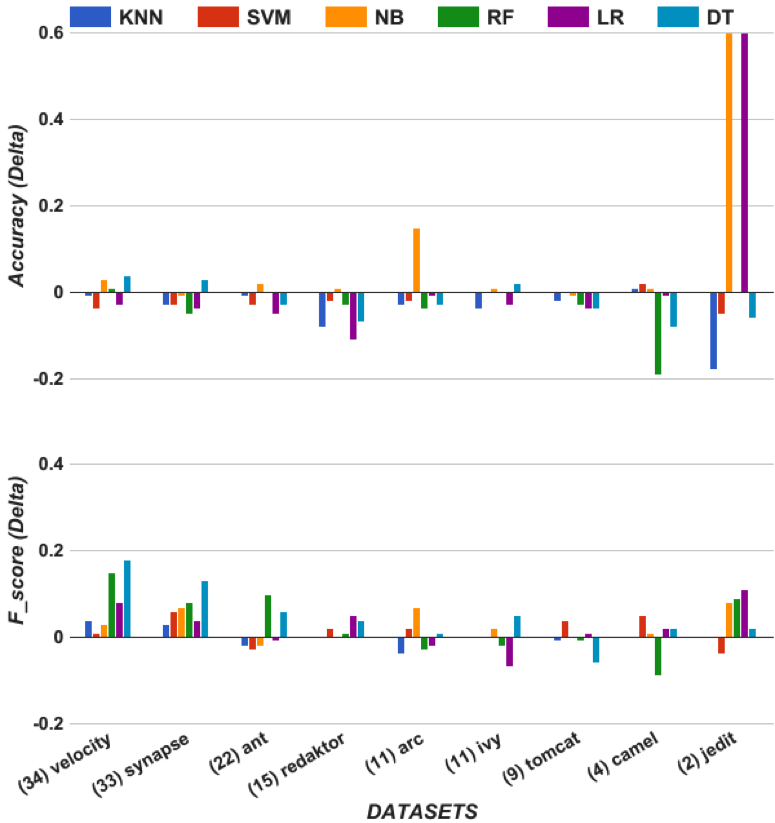
\includegraphics[width=.95\linewidth]{./fig/acc_f_tuned.png}
%     \end{minipage}%
%     \caption{SMOTUNED improvement over SMOTE. Legends represent the classifiers mentioned in \tion{classes}}
%     \label{fig:threats}
% \vspace{-0.5cm}
% \end{figure}



\section{Conclusion}
\label{sect:conclusion}




% %3681 modules, 1034314 lines of code
% We have shown that  prior ranking studies were incomlete (too few performance measures, too little exploration of class imbalance issues). Hence, this paper 

% Hence this paper. Prior work offered conflicting results on the benefits of class imbalance tools like SMOTE. We conjectted that this  as due to different data sets needed different params,. Hence, we designed SMOTUNED

% when applied, spectacualrly lare improvements in AUC and recall with
% little harmful side-effects seen in precision or false alarms. These are some of the alrgeest imrpovments we have ever seen, even after years of work in this field. Several aspects of this improvments are noteworthy:

% - largest yet seen

% - our results are stable across many data sets, and performance measures. this is unusual since results in this field are usually much more variable.

% - large improvements not associated with larger imbalances. STRANGE!

% - overtuned established wisdom in the field

% - did not matter wheat learners was used

% So we conclude that ``better data'' does better than ``better data miners''. In future need to study more the data being explored, rather than the data miner used to explore that data. boats on an ocena

% we also conclude that many prior ranking studies of defect predictors
% have to be revisited, this time exploring better methods for data pre-processing. 

Prior work on ranking studies tried to improve software analytics by selecting better learners.
Our results show that there may be {\em more} benefit in exploring data pre-processors like {\smb}:
\bi
\item
We found  that no  learner  was  usually  
``best''  
across all  data  sets  and  all  evaluation  criteria. 
\item 
On the other hand, across the same data sets,
{\smb} was  consistently  used  by  whatever  learner  was  found  to  be ``best'' in the  AUC/recall results;
\item
And in the precision+false alarm results, there was little evidence against the use of {\smb}.
\ei
That is, creating better training data  (using techniques like {\smb}) may be  more important than  the  subsequent  choice  of a classifier.


\noindent
As to specific recommendations,
we suggest that:
\bi
 %\item Previous studies~\cite{ghotra2015revisiting,tantithamthavorn2016automated} have mostly reported on only 1 evaluation goal, but we reported on many.
 \item Any prior ranking study  which did not  study the effects of data pre-processing needs to be analyzed again.
 \item Any future such ranking study should include a {\sma}-like
 pre-processor.
 \item {\sma} should not be used with its default parameters.
 For each new data set,
{\sma} should be used with some automatic parameter tuning tool in
order to find the best parameters for that data set.
\item {\smb} should be considered for parameter tuning.
\item Ideally, {\smb} should be tuned using the evaluation criteria used to assess the final predictors.
However, if there is not enough CPU to run {\smb} for each new evaluation criteria, {\smb} can be tuned using AUC.
\ei
% In the future, we plan to work on other similar issues like:
% \bi
%  \item Tuning SMOTE and learners at the same time and comparing against the results of No SMOTE, SMOTE, and SMOTUNED.
%  \item Predicting the quantities of defects which is regression based model rather having a binary based classification model with tuning.
% \ei
One surprise from our results was that the performance improvements associated with {\smb} were not substantially different between balanced and unbalanced data sets.
 {\sma} was originally proposed as a method to correct class imbalance; e.g. when the target class is only a small fraction of the instances in the training data.
 Yet our results show that {\sma} (and {\smb}) is also useful for balanced data sets (and best results come from automatically tuning the control parameters of {\sma}). We conjecture that {\smb}
is best viewed as a   {\em signal amplifier} for regions of the data where the quality signal is weak  (e.g. sparse regions with very little data between far-flung outliers).


 


Finally, while the above results were focused on classifiers exploring defect prediction, we note that many other software analytics
tasks use classifiers:
\bi
\item Predicting Github issue close time~\cite{jones17};
\item As a pre-processor to build the tree used to 
infer quality improvement plans~\cite{krishna2017less};
\item Non-parametric sensitivity analysis~\cite{menzies2000practical};
\item Etc.
\ei
That is, potentially, {\smb} is  a sub-routine that could improve many software analytics tasks. This could be a highly fruitful direction for future research.

\section*{Acknowledgements}
The work is partially funded by
%NSF awards \#1506586  and \#1302169.
funding source (blinded for review).

\balance

\bibliographystyle{abbrv}

%\bibliographystyle{ACM-Reference-Format}
\medskip
 \bibliography{main}


\end{document}





% To tackle the variations available among classifiers, some studies suggested to tune the learners to find the best parameter settings~\cite{tantithamthavorn2016automated, fu2016tuning}.  Both the studies report how performance of a defect predictor is dependent on the parameter settings of the predictors and recommends to use automated ways to tune the predictors.
% %According to them every dataset comes with different attributes and with different configurable learners, and we can not use a parameter settings found out by previous studies. Every time a defect prediction learner is used it is recommended to find automatic ways to tune them. 
% Recent studies~\cite{fu2016tuning, agrawal2016wrong} endorse DE as a method to perform automated tuning (also known as hyperparameter optimization). This was the motivation to use an automatic method like DE to
% tune the settings of SMOTE.

% In terms of the paper with most influential work,
% our experimental methods to select which learners to pick are informed 
% by  Ghotra et al.~\cite{ghotra2015revisiting} on ``Revisiting the impact of classification techniques on the performance of defect prediction models''. To 
% compare  the  performance  of  defect prediction  models,  they  used  the  Area  Under  the Receiver Operating Characteristic (ROC) Curve (AUC), which plots  false  positive  rate  against   true  positive rate. We denote this as $AUC\ (pf, recall)$. 

% They ran the Scott-Knott test~\cite{jelihovschi2014scottknott} to group classification techniques into statistically distinct ranks (in Table 9 of ~\cite{ghotra2015revisiting}). Ghotra et al. divided the classifers into four bands and we use 2 each from first three bands to show that ranking of these classifiers change when we consider data imbalance effects. And these 4 bands of classifiers provided by Ghotra et al., is for open source datasets available from PROMISE~\cite{promiserepo}. NASA corpus was not studied as there is data quality issue as assessed by Shepperd et al.~\cite{shepperd2013data}. From Ghotra et al., we studied Support Vector Machines (SVM - Linear Kernel), Linear Regression (LR), Naive Bayes (NB), K Nearest Neighbors (KNN - $K=8$), Decision Trees (DT - CART, Split Criteria=Entropy) and Random Forests (RF - Split Criteria=Entropy) for defect prediction.



%  false alarms and with only minimal changes to false alar,s.
% The first thing to note in are the very large improvements in AUC and recall and the 
% very small changes to precision and false alarm:

% \bi
% \item The AUC delta results are some of the largest we have ever seen, for any treatment, in any defect prediction paper.
% \item The precision delta results are particularly small;
% i.e. 


% That is, Figure~\ref{fig:tuned} offers much evidence that SMOTUNED is useful


%   \subsection{RQ2: In terms of the performance of defect predictors, are there benefit in tuning the default parameters of SMOTE for each new data set?}

%  \begin{lesson}For defect data, {\sma} has adverse effect on 
%  precision, modest improvements for AUC (pf, recall) and large improvements in recall.
%  \end{lesson}

 

%  \textbf{RQ2}: \textbf{Can {\smb} achieve better results?} 
 
%  \begin{lesson}For defect data, {\smb}  
%  offered    improvements over {\sma} for recall
%  and dramatic improvements for AUC (pf, recall).
%  \end{lesson}
 
%  \textbf{RQ3}: \textbf{Does hyperparameter optimization lead to different optimal configurations for different datasets?} 
 
%  \begin{lesson}Yes. DE finds different ``best'' parameter settings for {\sma} on different datasets.
%  \end{lesson}
%   This is an important result
%   since it means
%   reusing tunings suggested  by  any other  previous study  for a dataset different from the one under study is \underline{{\em not}} recommended. Instead,  it is better to
%       use automatic tuning  methods  to find the best tuning parameters for the 
%       under study dataset.
      
%       Note that
%  before we demand that tuning should be a
%  standard for all analytics task,
%  we must assess the practicality of that
%  proposal. This leads to the next question:
 
%   \textbf{RQ4}: \textbf{Is tuning 
%   impractically
%   slow?} 
 
%  \begin{lesson}Tuning using DE makes training runtimes about twenty times slower, but given
%  the large performance improvements,
%  the extra effort is justifiable. \end{lesson}
 
 



% \subsection{\textbf{RQ1: Is standard ``off-the-shelf'' SMOTE preprocessing method useful for defect prediction?}}

% Figure~\ref{fig:stats} shows Scott-Knott analysis of No-Smote, SMOTE and SMOTUNED. Each subfigure shows the 4 different evaluation measures (mentioned in \tion{measure}) compared with 6 learners (mentioned in \tion{classes}). The columns are sorted in the decreasing percentage of defective classes from left to right.

% For many of the results in Figure~\ref{fig:stats}, the changes
% resulting from applying SMOTE are very modest. There are improvements in AUC and recall with SMOTE over No-Smote but the improvements are not big as compared with SMOTUNED.

% The two consistent exceptions to that pattern are:
% \bi
% \item 
% SMOTE is not preferred when we can achieve better performance with SMOTUNED
% \item 
% Occasionally, SMOTE leads to poor performance in precision and false alarm but in many cases, they are not statistically significant different as shown in Figure~\ref{fig:stats}.  
% \ei

% We are not seeing any improvement in precision nor decrement in false alarm, the reason behind this is its maths. Zhang's~\cite{menzies2007problems} equation as given by Zhang can be rearranged to:
% \[
%   \mathit{pf}=  \frac{pos}{neg} *\frac{1-\mathit{prec}}{\mathit{prec}}* \mathit{pd}\]

% Pos and neg in the equation represents the imbalance ratio among the data samples. When we consider, pos to neg ratio and $prec$ constant, we are seeing there is direct relation between $pf$ and $pd$. So if pd is improved, we are bound to see improvement in pf. AUC is used to balance out this relation between pf and pd recommending to have higher AUC. On the other hand with prec, pf has indirect relation and since pf is increasing which is making prec improvements negligible.

% %  False positives (from Figure~\ref{fig:cmatrix}) do not get reduced after applying SMOTE. SMOTE generates synthetic examples within defective data samples and its neighbors making more denser region for positive samples. So if there are any actual negative samples surrounding these denser regions will now get wrongly classified as positive by learners. 

% % Based on these results,  we can best recommend SMOTE when:
% % \bi
% % \item Trying to improve recall
% % for imbalanaced datasets;
% % \item
% % Using NB or Random Forests.
% % \ei

% % For SMOTUNED improvement over SMOTE (figure~\ref{fig:tuned}), AUC values are shown in subfigure~\ref{fig:tuned}a. Redaktor dataset is selected from X-axis, and yellow bar represents NB which corresponds to about $-0.08$ AUC value. This denotes that NB performed worse by tuning the parameters of SMOTE. The original parameter settings of SMOTE worked the best. On the other hand for the same dataset, KNN (which is represented in dark blue bar) shows the AUC value of $0.35$. This shows KNN outperformed the ``off-the-shelf'' SMOTE when tuned using DE.



% % By looking at the results of AUC from figure~\ref{fig:untuned}a, only 4 bars are negative, and rest all the remaining 50 bars (in total 9 datasets with 6 learners in each) have  positive effect by using SMOTE as a preprocessing method. We are seeing a maximum improvement of about 30\%. These improvements are quite modest as to ignore the importance of SMOTE.

% % Results for precision (in figure~\ref{fig:untuned}b), are not much interesting, but the decrease in precision value is not that arduous except for the redaktor dataset. Though we will not recommend using SMOTE whenever we want higher precision value. Since precision is decreased using SMOTE, it was expected to have increased false alarm \cite{menzies2007problems} and the same is observed from figure~\ref{fig:untuned}d. There is an increase in error among false positives but the increase is very minimal.

% % As for recall (figure~\ref{fig:untuned}c), only 4 bars are negative, and rest all the remaining 50 bars (in total 9 datasets with 6 learners in each) have positive effect by using SMOTE. We are seeing a maximum improvement of about 60\%. These improvements are quite steep as to ignore the importance of SMOTE at any point for any learner. It is also observed that performance keeps increasing as target class becomes more minor and minor. This is what was expected after applying SMOTE to imbalance datasets.

% \noindent
% Summarizing the above:
% \begin{lesson1}
% We recommend SMOTE for improving recall, but SMOTE can,
% sometimes, adversely affect
% precision.
% \end{lesson1}


% \subsection{\textbf{RQ2: Can SMOTUNED achieve better results?}}

% Figure~\ref{fig:tuned} shows the results
% after applying SMOTUNED. The
% plot shows the {\em delta} between
% the results obtained by SMOTUNED over SMOTE.

% For subfigures (AUC, Recall and Precision):
% \bi
% \item 
% {\em Larger} y-values
% are {\em better} 
% \item
% If the y-value goes {\em negative}, then the corresponding learner trained on SMOTUNED data is {\em worse} than learner learnt on SMOTE data respectively. 
% \ei
% For the false alarms, the
% plots must be interpreted differently:
% \bi
% \item
% {\em Larger} y-values are {\em worse};
% \item
% If the y-value goes {\em positive} then the corresponding learner trained on SMOTUNED data is {\em worse} than learner learnt on SMOTE data respectively.
% \ei

% The benefit of SMOTUNED's tunings is clearly evident in the AUC results of  Figure~\ref{fig:tuned}a:
% all learners show large performance improvements. And from the Scott-Knott test shown in Figure~\ref{fig:stats}, SMOTUNED always have significantly best results for AUC. For recall, in most learners either SMOTE or SMOTUNED are significantly the same, or SMOTUNED performed better. 
% Better yet,  as
% shown in
% Figure~\ref{fig:stats}, for precision and false alarm, SMOTUNED does
% not adversely effect false alarm and precision as most of the times No-SMOTE, SMOTE, and SMOTUNED are significantly the same.


% At first glance, SMOTUNED's effects on recall seem strange since they are
% {\em better} for the more balanced left-hand-side datasets of
% Figure~\ref{fig:tuned}c.  But recall from the above that SMOTE had less
% of an effect on those left-hand-side datasets. That is, what we are seeing
% here is that:
% \bi
% \item
% SMOTUNED works often as well as SMOTE for imbalanced datasets;
% \item
% SMOTUNED offers additional benefits for datasets that are not greatly
% imbalanced.
% \ei


% % results are dramat
% % Now when we look at the results of AUC from figure~\ref{fig:tuned}a, only 1 bar is negative, and rest all the remaining 53 bars (in total 9 datasets with 6 learners in each) have  positive effect after when we tune the parameters of SMOTE. We are seeing a maximum improvement of about 70\% and on an average 50\% for each learner in all datasets. These improvements are quite steep in nature and just to remind you that these results are improvement over SMOTE. If we combine the results, then we can surely say to tune the parameters of SMOTE and train using any learner, we will get atleast 100\% improvement in most cases.

% % We are seeing the similar trend of results for precision (in figure~\ref{fig:tuned}b), just like in Figure~\ref{fig:untuned}b, that even after tuning for precision, we are not seeing much improvement. Though we definitely improved precision slightly than SMOTE but the increment is not that large to recommend SMOTUNED or SMOTE. And even after trying to minimise the false alarm (figure~\ref{fig:tuned}d) value, DE could not find a good parameter setting.

% % As for recall (figure~\ref{fig:untuned}c), only 5 bars are negative, and rest all the remaining 49 bars (in total 9 datasets with 6 learners in each) have either positive effect or no effect after tuning. We are seeing a maximum improvement of about 65\% but the average improvement is close to 15\% for each classifiers in all datasets. But these improvements combined with SMOTE suggest that we should always tune SMOTE whenever the goal is to achieve higher recall.

% In summary:

% \begin{lesson1}
%     For defect data, SMOTUNED  
%  offers   some  improvements over SMOTE for recall
%  and dramatic improvements for AUC (pf, recall).
%  The effects on precision and false alarm are similar to SMOTE.
% \end{lesson1}

% %Based on these results, we strongly recommend SMOTUNED for handling not just unbalanced datasets but, in fact, for all datasets.

% \subsection{\textbf{RQ3: Does hyperparameter optimization lead to different optimal configurations for different datasets?}}

% Figure \ref{fig:para} represents the parameter variations when we tuned to maximize the recall. These parameter settings are found by each learner for that dataset.
% On display in each set of vertical bars are
% the median values generated across 25 evaluations.
% Also, shown are
% the inter-quartile range (IQR) of those tunings (the IQR is the 75th-25th percentile values and is a non-parametric measure of variation
% around the median value). Note that in Figure \ref{fig:para}b, IQR=0 for  ant dataset where tuning always converged on the same final value. That shows that the maximum score of recall is reached when $m=50$. No other parameter setting found out to be useful by DE.

%   These figures
% show how tuning selects the different ranges  of
% parameters.
% Some of the above numbers are far from the standard values; e.g. Chawla et al.~\cite{chawla2002smote} recommend using $k=5$ neighbors yet in our datasets, best results were seen using $k \approx 13$. On other hand it was suggested to use $m=900$ by ~\cite{pears2014synthetic}.
% Clearly,
% best results from tuning
% vary with each dataset.

% Clearly:
% \begin{lesson1}
%     Yes. DE finds different ``best'' parameter settings for SMOTUNED on different datasets.
% \end{lesson1}
%  That is,  reusing tunings  suggested  by  any other  previous study  for any dataset is \underline{{\em not}} recommended. Instead,  it is better to
%       use  automatic  tuning  methods  to find the best tuning parameters for the current dataset.
      

% \subsection{\textbf{RQ4: Is tuning impractically slow?}}

% Search-based SE methods can be very slow. Wang et al.~\cite{wang2013searching} once needed 15
% years of CPU time to find and verify the tunings required for software
% clone detectors. Sayyad et al.~\cite{sayyad2013scalable} routinely used
% $10^6$ evaluations (or more) of their models in order to extract
% products from highly constrained product
% lines. Hence, before recommending any
% search-based method, it is wise to consider the runtime cost of that
% recommendation.


%  Figure~\ref{runtime} shows,  in circle and square markers, the
%   runtimes required to run SMOTE and SMOTUNED respectively and the numbers shown in the graph is an average over 6 learners.  The
%   longer runtimes (in square) include the times required for DE to find
%   the tunings and this is a disadvantage with SMOTUNED. Figure~\ref{runtime} shows SMOTE reporting all the measures in the shown time. On the other hand, here SMOTUNED reports runtimes when trying to maximize recall. If it has to provide all the other 3 measures as well, it would take 3 times more than the above number which is not recommended in a real world scenario. 
  
%   The work around would be is to try maximizing SMOTUNED for AUC tuning goal. AUC represents the area under the curve for pf (false alarm) and recall. When AUC improves, the heuristic is that false alarm must be getting lower and recall must be improving. And if false alarm is getting lower then precision is improving as well~\cite{menzies2007data}. We report results of AUC, Precision, Recall and False alarm in Figure~\ref{fig:auc} when we tried maximizing only AUC. We are seeing a similar conclusions as answered in our RQ2. 
  
%   This additional result shows that, tuning slows down the training by a factor of up to
%   twenty for 1 goal (which is very close to our theoretical prediction) but the improvements achieved are quite advantageous.

% \begin{lesson1}
%     Tuning with DE makes training about twenty times slower, but the improvements in performance with respect to AUC and recall justifies the extra time required for training.
% \end{lesson1}

 
%  As discussed above, the default parameters for
%  SMOTE are $k,m,r = 5,100,2$.
%   Figure~\ref{fig:para} shows the range of parameters
%  found by SMOTE across  nine data sets for the 25 repeats of our cross-validation procedure.
%  All the results in this figure are {\em within-measure assessment} results; i.e.
%  here, we SMOTUNED trains of some performance measure and then we only collect performance for that performance measure in the test set.
 
 
%  In  Figure~\ref{fig:para}, {\em median} is the 50th percentile
%  value and {\em IQR} is the (75-25)th percentile
%  (IQR is a non-parametric analgoue of variance).
%  As can be seen in Figure~\ref{fig:para}, most of the learned parameter are far from the default values:
%  \bi
%  \item 
%  Median $k$ value was never less than 11;
%  \item
%  Median m value of often twice or half the default value used in SMOTE;
%  \item
%  The $r$ value used in the distance function was never 2. Rather, it was usually 3.
%  \ei
%  Hence,  our answer to {\bf RQ1} is ``no'': the use of off-the-shelf SMOTE should be deprecated. 
   



% \subsection {RQ2: What are there benefit in tuning the default parameters of SMOTE for each new data set?}

% Figure~\ref{fig:tuned} shows the performance delta of the {\em within-measure assessment rig}.
% Recall that when this rig applies SMOTUNED, it optimizes for performance measure
% \[M_i \in \{ 
% \mathit{recall},
% \mathit{precision}, 
% \mathit{false\; alarm},
% \mathit{AUC}
% \}
% \]
% after which it uses the {\em same} performance measure
% when processing test data.
% As shown in Figure~\ref{fig:tuned}, 
% SMOTUNED achieves large AUC and recall improvements
% without
%  damaging precision and  with only minimal changes
%  to false alarms. Special note should be take of the  AUC improvements- these are the largest improvements
%  we have yet seen, for any prior treatment of defect prediction data.

% Figure~\ref{fig:stats} offers a statistical 

 
%  false alarms and with only minimal changes to false alar,s.
% The first thing to note in are the very large improvements in AUC and recall and the 
% very small changes to precision and false alarm:

% \bi
% \item The AUC delta results are some of the largest we have ever seen, for any treatment, in any defect prediction paper.
% \item The precision delta results are particularly small;
% i.e. 


% That is, Figure~\ref{fig:tuned} offers much evidence that SMOTUNED is useful


%   \subsection{RQ2: In terms of the performance of defect predictors, are there benefit in tuning the default parameters of SMOTE for each new data set?}

%  \begin{lesson}For defect data, {\sma} has adverse effect on 
%  precision, modest improvements for AUC (pf, recall) and large improvements in recall.
%  \end{lesson}



% \begin{figure*}[!htbp]
% \begin{minipage}{.5\linewidth}
% \centering
%         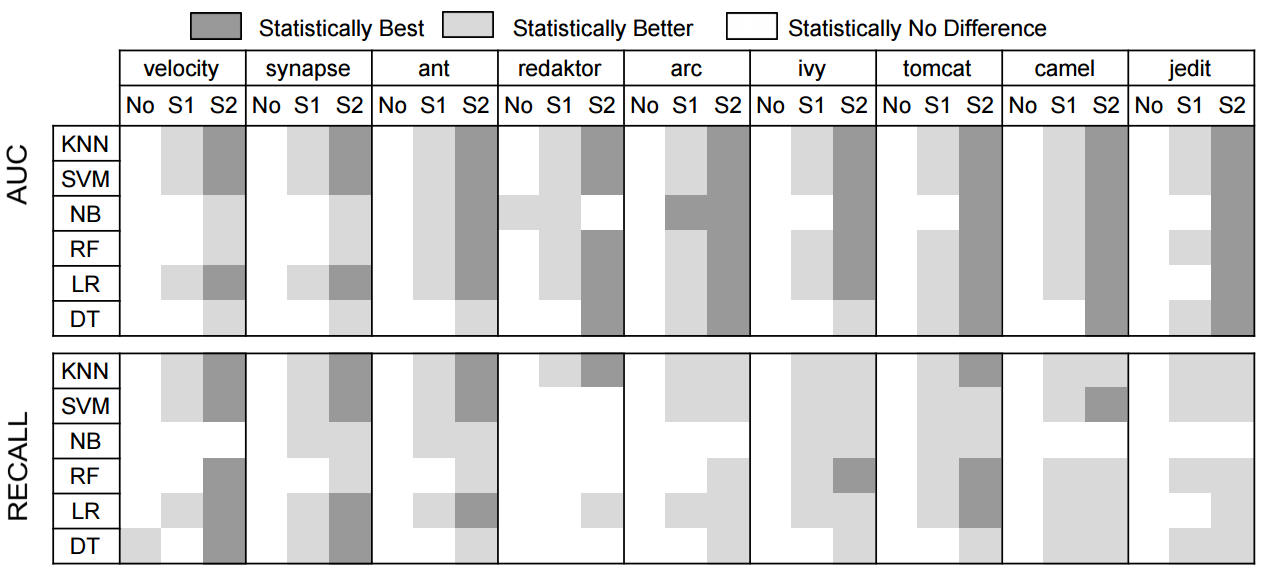
\includegraphics[width=.9\linewidth]{./fig/AUC_recall.png}
%             \end{minipage}%
% \begin{minipage}{.5\linewidth}
%         \centering
%         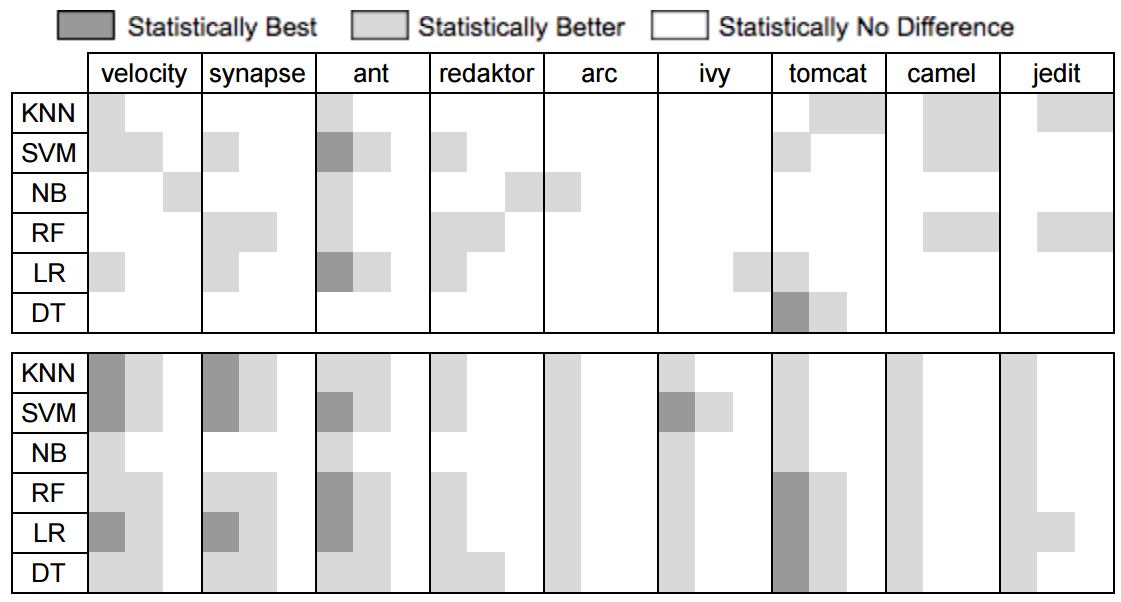
\includegraphics[width=.9\linewidth]{./fig/prec_pf.png}
%     \end{minipage}%
%     \caption{Scott Knott analysis of No-SMOTE, SMOTE and SMOTUNED. The column headers are denoted as No for No-SMOTE, S1 for SMOTE and S2 for SMOTUNED. $(\ast)$ Mark represents the best learner combined with its techniques.}
%     \label{fig:stats}
% \vspace{-0.2cm}
% \end{figure*}

%  \textbf{RQ2}: \textbf{Can {\smb} achieve better results?} 
 
%  \begin{lesson}For defect data, {\smb}  
%  offered    improvements over {\sma} for recall
%  and dramatic improvements for AUC (pf, recall).
%  \end{lesson}
 
%  \textbf{RQ3}: \textbf{Does hyperparameter optimization lead to different optimal configurations for different datasets?} 
 
%  \begin{lesson}Yes. DE finds different ``best'' parameter settings for {\sma} on different datasets.
%  \end{lesson}
%   This is an important result
%   since it means
%   reusing tunings suggested  by  any other  previous study  for a dataset different from the one under study is \underline{{\em not}} recommended. Instead,  it is better to
%       use automatic tuning  methods  to find the best tuning parameters for the 
%       under study dataset.
      
%       Note that
%  before we demand that tuning should be a
%  standard for all analytics task,
%  we must assess the practicality of that
%  proposal. This leads to the next question:
 
%   \textbf{RQ4}: \textbf{Is tuning 
%   impractically
%   slow?} 
 
%  \begin{lesson}Tuning using DE makes training runtimes about twenty times slower, but given
%  the large performance improvements,
%  the extra effort is justifiable. \end{lesson}
 
 



% \subsection{\textbf{RQ1: Is standard ``off-the-shelf'' SMOTE preprocessing method useful for defect prediction?}}

% Figure~\ref{fig:stats} shows Scott-Knott analysis of No-Smote, SMOTE and SMOTUNED. Each subfigure shows the 4 different evaluation measures (mentioned in \tion{measure}) compared with 6 learners (mentioned in \tion{classes}). The columns are sorted in the decreasing percentage of defective classes from left to right.

% For many of the results in Figure~\ref{fig:stats}, the changes
% resulting from applying SMOTE are very modest. There are improvements in AUC and recall with SMOTE over No-Smote but the improvements are not big as compared with SMOTUNED.

% The two consistent exceptions to that pattern are:
% \bi
% \item 
% SMOTE is not preferred when we can achieve better performance with SMOTUNED
% \item 
% Occasionally, SMOTE leads to poor performance in precision and false alarm but in many cases, they are not statistically significant different as shown in Figure~\ref{fig:stats}.  
% \ei

% We are not seeing any improvement in precision nor decrement in false alarm, the reason behind this is its maths. Zhang's~\cite{menzies2007problems} equation as given by Zhang can be rearranged to:
% \[
%   \mathit{pf}=  \frac{pos}{neg} *\frac{1-\mathit{prec}}{\mathit{prec}}* \mathit{pd}\]

% Pos and neg in the equation represents the imbalance ratio among the data samples. When we consider, pos to neg ratio and $prec$ constant, we are seeing there is direct relation between $pf$ and $pd$. So if pd is improved, we are bound to see improvement in pf. AUC is used to balance out this relation between pf and pd recommending to have higher AUC. On the other hand with prec, pf has indirect relation and since pf is increasing which is making prec improvements negligible.

% %  False positives (from Figure~\ref{fig:cmatrix}) do not get reduced after applying SMOTE. SMOTE generates synthetic examples within defective data samples and its neighbors making more denser region for positive samples. So if there are any actual negative samples surrounding these denser regions will now get wrongly classified as positive by learners. 

% % Based on these results,  we can best recommend SMOTE when:
% % \bi
% % \item Trying to improve recall
% % for imbalanaced datasets;
% % \item
% % Using NB or Random Forests.
% % \ei

% % For SMOTUNED improvement over SMOTE (figure~\ref{fig:tuned}), AUC values are shown in subfigure~\ref{fig:tuned}a. Redaktor dataset is selected from X-axis, and yellow bar represents NB which corresponds to about $-0.08$ AUC value. This denotes that NB performed worse by tuning the parameters of SMOTE. The original parameter settings of SMOTE worked the best. On the other hand for the same dataset, KNN (which is represented in dark blue bar) shows the AUC value of $0.35$. This shows KNN outperformed the ``off-the-shelf'' SMOTE when tuned using DE.



% % By looking at the results of AUC from figure~\ref{fig:untuned}a, only 4 bars are negative, and rest all the remaining 50 bars (in total 9 datasets with 6 learners in each) have  positive effect by using SMOTE as a preprocessing method. We are seeing a maximum improvement of about 30\%. These improvements are quite modest as to ignore the importance of SMOTE.

% % Results for precision (in figure~\ref{fig:untuned}b), are not much interesting, but the decrease in precision value is not that arduous except for the redaktor dataset. Though we will not recommend using SMOTE whenever we want higher precision value. Since precision is decreased using SMOTE, it was expected to have increased false alarm \cite{menzies2007problems} and the same is observed from figure~\ref{fig:untuned}d. There is an increase in error among false positives but the increase is very minimal.

% % As for recall (figure~\ref{fig:untuned}c), only 4 bars are negative, and rest all the remaining 50 bars (in total 9 datasets with 6 learners in each) have positive effect by using SMOTE. We are seeing a maximum improvement of about 60\%. These improvements are quite steep as to ignore the importance of SMOTE at any point for any learner. It is also observed that performance keeps increasing as target class becomes more minor and minor. This is what was expected after applying SMOTE to imbalance datasets.

% \noindent
% Summarizing the above:
% \begin{lesson1}
% We recommend SMOTE for improving recall, but SMOTE can,
% sometimes, adversely affect
% precision.
% \end{lesson1}


% \subsection{\textbf{RQ2: Can SMOTUNED achieve better results?}}

% Figure~\ref{fig:tuned} shows the results
% after applying SMOTUNED. The
% plot shows the {\em delta} between
% the results obtained by SMOTUNED over SMOTE.

% For subfigures (AUC, Recall and Precision):
% \bi
% \item 
% {\em Larger} y-values
% are {\em better} 
% \item
% If the y-value goes {\em negative}, then the corresponding learner trained on SMOTUNED data is {\em worse} than learner learnt on SMOTE data respectively. 
% \ei
% For the false alarms, the
% plots must be interpreted differently:
% \bi
% \item
% {\em Larger} y-values are {\em worse};
% \item
% If the y-value goes {\em positive} then the corresponding learner trained on SMOTUNED data is {\em worse} than learner learnt on SMOTE data respectively.
% \ei

% The benefit of SMOTUNED's tunings is clearly evident in the AUC results of  Figure~\ref{fig:tuned}a:
% all learners show large performance improvements. And from the Scott-Knott test shown in Figure~\ref{fig:stats}, SMOTUNED always have significantly best results for AUC. For recall, in most learners either SMOTE or SMOTUNED are significantly the same, or SMOTUNED performed better. 
% Better yet,  as
% shown in
% Figure~\ref{fig:stats}, for precision and false alarm, SMOTUNED does
% not adversely effect false alarm and precision as most of the times No-SMOTE, SMOTE, and SMOTUNED are significantly the same.


% At first glance, SMOTUNED's effects on recall seem strange since they are
% {\em better} for the more balanced left-hand-side datasets of
% Figure~\ref{fig:tuned}c.  But recall from the above that SMOTE had less
% of an effect on those left-hand-side datasets. That is, what we are seeing
% here is that:
% \bi
% \item
% SMOTUNED works often as well as SMOTE for imbalanced datasets;
% \item
% SMOTUNED offers additional benefits for datasets that are not greatly
% imbalanced.
% \ei


% % results are dramat
% % Now when we look at the results of AUC from figure~\ref{fig:tuned}a, only 1 bar is negative, and rest all the remaining 53 bars (in total 9 datasets with 6 learners in each) have  positive effect after when we tune the parameters of SMOTE. We are seeing a maximum improvement of about 70\% and on an average 50\% for each learner in all datasets. These improvements are quite steep in nature and just to remind you that these results are improvement over SMOTE. If we combine the results, then we can surely say to tune the parameters of SMOTE and train using any learner, we will get atleast 100\% improvement in most cases.

% % We are seeing the similar trend of results for precision (in figure~\ref{fig:tuned}b), just like in Figure~\ref{fig:untuned}b, that even after tuning for precision, we are not seeing much improvement. Though we definitely improved precision slightly than SMOTE but the increment is not that large to recommend SMOTUNED or SMOTE. And even after trying to minimise the false alarm (figure~\ref{fig:tuned}d) value, DE could not find a good parameter setting.

% % As for recall (figure~\ref{fig:untuned}c), only 5 bars are negative, and rest all the remaining 49 bars (in total 9 datasets with 6 learners in each) have either positive effect or no effect after tuning. We are seeing a maximum improvement of about 65\% but the average improvement is close to 15\% for each classifiers in all datasets. But these improvements combined with SMOTE suggest that we should always tune SMOTE whenever the goal is to achieve higher recall.

% In summary:

% \begin{lesson1}
%     For defect data, SMOTUNED  
%  offers   some  improvements over SMOTE for recall
%  and dramatic improvements for AUC (pf, recall).
%  The effects on precision and false alarm are similar to SMOTE.
% \end{lesson1}

% %Based on these results, we strongly recommend SMOTUNED for handling not just unbalanced datasets but, in fact, for all datasets.

% \subsection{\textbf{RQ3: Does hyperparameter optimization lead to different optimal configurations for different datasets?}}

% Figure \ref{fig:para} represents the parameter variations when we tuned to maximize the recall. These parameter settings are found by each learner for that dataset.
% On display in each set of vertical bars are
% the median values generated across 25 evaluations.
% Also, shown are
% the inter-quartile range (IQR) of those tunings (the IQR is the 75th-25th percentile values and is a non-parametric measure of variation
% around the median value). Note that in Figure \ref{fig:para}b, IQR=0 for  ant dataset where tuning always converged on the same final value. That shows that the maximum score of recall is reached when $m=50$. No other parameter setting found out to be useful by DE.

%   These figures
% show how tuning selects the different ranges  of
% parameters.
% Some of the above numbers are far from the standard values; e.g. Chawla et al.~\cite{chawla2002smote} recommend using $k=5$ neighbors yet in our datasets, best results were seen using $k \approx 13$. On other hand it was suggested to use $m=900$ by ~\cite{pears2014synthetic}.
% Clearly,
% best results from tuning
% vary with each dataset.

% Clearly:
% \begin{lesson1}
%     Yes. DE finds different ``best'' parameter settings for SMOTUNED on different datasets.
% \end{lesson1}
%  That is,  reusing tunings  suggested  by  any other  previous study  for any dataset is \underline{{\em not}} recommended. Instead,  it is better to
%       use  automatic  tuning  methods  to find the best tuning parameters for the current dataset.
      

% \begin{figure}[!htbp]
%   \captionsetup{justification=centering}
%   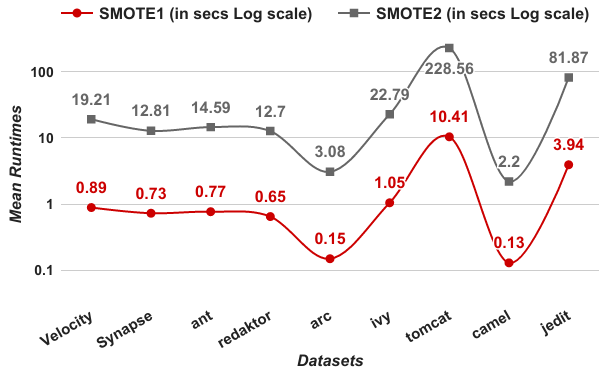
\includegraphics[width=\linewidth]{./fig/runtimes.png}
%   \caption{Datasets vs Runtimes. Note that the numbers
%   shown here at the total times for running six learners through a 5*5cross-validation. Hence, for mean
%   runtimes for one learner, {\em divide} these numbers by 6*5*5=150.}
%   \label{runtime}
% \vspace{-0.7cm}
% \end{figure}


% \subsection{\textbf{RQ4: Is tuning impractically slow?}}

% Search-based SE methods can be very slow. Wang et al.~\cite{wang2013searching} once needed 15
% years of CPU time to find and verify the tunings required for software
% clone detectors. Sayyad et al.~\cite{sayyad2013scalable} routinely used
% $10^6$ evaluations (or more) of their models in order to extract
% products from highly constrained product
% lines. Hence, before recommending any
% search-based method, it is wise to consider the runtime cost of that
% recommendation.


%  Figure~\ref{runtime} shows,  in circle and square markers, the
%   runtimes required to run SMOTE and SMOTUNED respectively and the numbers shown in the graph is an average over 6 learners.  The
%   longer runtimes (in square) include the times required for DE to find
%   the tunings and this is a disadvantage with SMOTUNED. Figure~\ref{runtime} shows SMOTE reporting all the measures in the shown time. On the other hand, here SMOTUNED reports runtimes when trying to maximize recall. If it has to provide all the other 3 measures as well, it would take 3 times more than the above number which is not recommended in a real world scenario. 
  
%   The work around would be is to try maximizing SMOTUNED for AUC tuning goal. AUC represents the area under the curve for pf (false alarm) and recall. When AUC improves, the heuristic is that false alarm must be getting lower and recall must be improving. And if false alarm is getting lower then precision is improving as well~\cite{menzies2007data}. We report results of AUC, Precision, Recall and False alarm in Figure~\ref{fig:auc} when we tried maximizing only AUC. We are seeing a similar conclusions as answered in our RQ2. 
  
%   This additional result shows that, tuning slows down the training by a factor of up to
%   twenty for 1 goal (which is very close to our theoretical prediction) but the improvements achieved are quite advantageous.

% \begin{lesson1}
%     Tuning with DE makes training about twenty times slower, but the improvements in performance with respect to AUC and recall justifies the extra time required for training.
% \end{lesson1}

% Many factors might explain this {\em conclusion instability}. For example,
% different classifiers might be best at handled different issues in different data sets.
% Those issues   include:
% \be
% \item
% Class imbalance;
% \item
% Low data quality~\cite{shepperd2013data,van2009knowledge};
% \item
% The degree of data overlapping (represented
% as duplicates) among the classes; 
% \item
% Dataset shift (training and test
% data follow different distributions)~\cite{turhan2012dataset};
% \item
% Small sample sizes (relative to the space of possible software projects);
% \item
% Management of borderline examples~\cite{lopez2014importance,lopez2012analysis};
% \item
% The presence of irrelevant or redundant attributes~\cite{xu2016impact};
% \item
% See also the long list of other factors that might contribute to conclusion
% instability in Table~1 of reference~\cite{menzies2012special}.
% \ee
% In the experiments reported below, we only adjust one item on the above list:
% the degree of class imbalance in the training set. A remarkable feature
% of the results seen in  those results is the resulting {\em conclusion \underline{stability}}. Across multiple data sets and performance criteria and 
% classifiers, we find that best performance scores were always obtained
% using a class imbalance algorithm that tuned its own control parameters
% on a dataset-by-dataset basis. This makes us conjecture that:
% \bi
% \item Addressing the issue of class imbalance seems to  fix man of the other issues
% listed above. Alternatively, fixing  class imbalance is more
% important than fixing the other seven issues.
% \item
% Instead
% of asking ``what is the best classifier to apply to the data'' is less insightful than another question;
% i.e. ``how can we improve   our training data?''.
